%--------------------------------------%
\newpage

\textbf{\vspace{80pt}}
\title{
    \BTitr
    \center \Huge
    \begin{flushright}
        \textbf{معرفی}
    \end{flushright}
}
\textbf{\vspace{80pt}}

{
    \Large
    \lr{Direct3D 12} یک کتابخانه‌ی رندر (\lr{render}) برای نوشتن برنامه‌های گرافیکی سه بعدی با عملکرد بالا (\lr{high-performance}) با استفاده از سخت‌افزار گرافیکی مدرن بر روی پلتفرم‌های مختلف ویندوز 10 \lr{(Windows Desktop - Mobile - Xbox One)} است.
\lr{Direct3D} یک کتابخانه سطح پایین است، به این معنا که رابط برنامه‌نویسی کاربردی آن (\lr{API}) مدل‌سازی سخت‌افزار گرافیکی زیرینی را که کنترل می‌کند، بر عهده دارد.
بیشترین استفاده‌ی \lr{Direct3D} صنعت بازی‌سازی است که در آن موتور‌های رندرینگ سطح بالاتر بر روی \lr{Direct3D} ساخته می‌شوند.
با این حال، صنایع دیگر به گرافیک سه بعدی تعاملی با عملکرد بالا نیز نیاز دارند، مانند: تجسم پزشکی و علمی و بررسی‌های معماری.
علاوه بر این، با مجهز شدن هر رایانه شخصی جدید به یک کارت گرافیک مدرن، برنامه‌هایی که سه بعدی نیستند، شروع به استفاده از \lr{GPU} (واحد پردازش گرافیکی) برای سپردن محاسبات فشرده به کارت گرافیک کردند.
این کار به عنوان \lr{\textit{general purpose GPU computing}} شناخته می‌شود و رابط برنامه‌نویسی کاربردی \lr{Direct3D}، \lr{shader} محاسباتی را برای نوشتن برنامه‌های \lr{GPU} با اهداف عمومی ارائه می‌دهد.
اگرچه \lr{Direct3D 12} معمولاً با \lr{C++} برنامه‌نویسی می‌شود، تیم \lr{\href{https://sharpdx.org/}{SharpDX}} در حال کار بر روی بسته‌های \lr{.NET} هستند تا بتوانید از برنامه‌های مدیریت شده به این \lr{API} گرافیکی سه بعدی قدرتمند دسترسی داشته باشید.
}

{
    \Large
    این کتاب مقدمه‌ای بر برنامه‌نویسی گرافیک کامپیوتری تعاملی با استفاده از \lr{Direct3D 12} و تأکید بر توسعه بازی است. اصول برنامه‌نویسی \lr{Direct3D} و \lr{shader} را آموزش می‌دهد و پس از آن خواننده آماده می‌شود تا تکنیک‌های پیشرفته‌تری را یاد بگیرد.
    کتاب به سه بخش اصلی تقسیم شده است. بخش اول ابزار‌های ریاضی را توضیح می‌دهد که در این کتاب استفاده خواهد شد.
    بخش دوم نحوه پیاده‌سازی وظایف اساسی در \lr{Direct3D} مانند: مقداردهی اولیه، تعریف هندسه سه بعدی، راه‌اندازی دوربین‌ها، ایجاد رئوس، ایجاد پیکسل، ایجاد هندسه و محاسبه سایه زن، نورپردازی، بافت‌سازی، مخلوط کردن، شابلون‌سازی، و مفروش‌سازی را نشان می‌دهد.
    بخش سوم عمدتاً در مورد استفاده از \lr{Direct3D} برای پیاده‌سازی انواع تکنیک‌های جالب و جلوه‌های ویژه است، مانند کار با مش شخصیت‌های متحرک، برداشتن، نگاشت محیط، نقشه‌برداری معمولی، سایه‌های بلادرنگ، و انسداد محیط.
}

{
    \Large
    افراد مبتدی، بهتر است این کتاب را از ابتدا به انتها به صورت کامل بخوانند. فصل‌ها به گونه‌ای مرتب شده‌اند که با گذر از هر فصل، میزان سختی به تدریج افزایش می‌یابد. به این ترتیب، هیچ جهش ناگهانی در پیچیدگی متنها وجود ندارد که خواننده را سردرگم کند.
    به طور کلی، برای هر فصل، از تکنیک‌ها و مفاهیمی که در فصل‌های قبل گفته شده‌اند استفاده خواهیم کرد. بنابراین، مهم است که بر مطالب هر فصل تسلط داشته باشید.
    خوانندگانی که تجربه‌ی استفاده از \lr{Direct3D} را دارند، می‌توانند فصل‌های مورد علاقه خود را بخوانند. در نهایت، شاید از خود بپرسید که بعد از خواندن این کتاب چه نوع بازی‌هایی را می‌توانید توسعه دهید، پاسخ این سؤال را بهتر است با مرور این کتاب و مشاهده انواع برنامه‌های توسعه یافته به دست‌آورید.
    از این رو می‌توانید انواع بازی‌های را بر اساس تکنیک‌های آموزش داده شده در این کتاب و نبوغ خود تجسم کنید.
}

%--------------------------------------%
\newpage

\title{
    \LARGE
    \textbf{مخاطبان کتاب}
}\rullFillWithLine[0.5em]{1pt}
\textbf{\vspace{12pt}}

{
    \Large
    این کتاب با در نظر گرفتن سه مخاطب زیر طراحی شده است:
    \begin{enumerate}
        \item {برنامه‌نویسان سطح متوسط \lr{C++} که می‌خواهند مقدمه‌ای بر برنامه‌نویسی سه بعدی با استفاده از آخرین نسخه \lr{Direct3D} داشته باشند}
        \item {برنامه‌نویسان سه بعدی با تجربه که با \lr{API}‌ای غیر از \lr{DirectX} (به عنوان مثال، \lr{OpenGL}) کار کرده‌اند و می‌خواهند مقدمه‌ای برای \lr{Direct3D 12} داشته باشند}
        \item {برنامه‌نویسان با تجربه \lr{Direct3D} که مایل به یادگیری آخرین نسخه \lr{Direct3D} هستند}
    \end{enumerate}
}
\textbf{\vspace{25pt}}

\title{
    \LARGE
    \textbf{پیش نیاز ها}
} \rullFillWithLine[0.5em]{1pt}
\textbf{\vspace{12pt}}

{
    \Large
    لازم به ذکر است که این مقدمه‌ای بر \lr{Direct3D 12}، برنامه‌نویسی \lr{shader} و برنامه‌نویسی بازی‌های سه بعدی است و نمی‌توان از آن برای یادگیری برنامه‌نویسی کامپیوتر به صورت کلی استفاده کرد. بنابراین خواننده باید شرایط زیر را رعایت کند:
    \begin{enumerate}
        \item {\textbf{ریاضیات دبیرستان: } مثلاً جبر، مثلثات و توابع ریاضی}
        \item {\textbf{تجربه‌ی کار با \lr{Visual Studio}:} چگونگی ایجاد پروژه‌ها، اضافه کردن فایل‌ها و \lr{link} کردن کتابخانه‌های خارجی}
        \item {\textbf{\lr{C++} متوسط و مهارت‌های ساختار داده:} به عنوان مثال: تجربه‌ی کار با اشاره گر‌ها، آرایه‌ها، سربار اپراتور‌ها، لیست‌های پیوندی، وراثت و چند ریختی}
        \item {\textbf{آشنایی با برنامه‌نویسی ویندوز با \lr{Win32 API}} (مفید است اما لازم نیست)}
    \end{enumerate}
}
\textbf{\vspace{25pt}}

\title{
    \LARGE
    \textbf{ابزارها و سخت افزارهای توسعه مورد نیاز}
} \rullFillWithLine[0.5em]{1pt}
\textbf{\vspace{12pt}}

{
    \Large
    برای برنامه‌نویسی برنامه‌های \lr{Direct3D 12} به حداقل موارد زیر نیاز است:
    \begin{enumerate}
        \item {\lr{Windows 10}}
        \item {\lr{Visual Studio 2015} یا جدیدتر}
        \item {کارت گرافیکی که از \lr{Direct3D 12} پشتیبانی کند}
    \end{enumerate}
}

\textbf{\vspace{6pt}}
\begin{theo}{thm:pythagoras}
    \Large
    کانفیگ های استفاده شده از این کتاب طبق موارد زیر است:
    \lr{
        \begin{enumerate}
            \item {Windows 11 Pro 22H2 Build 22621.1992}
            \item {NVIDIA GeForce GTX 960m}
            \item {Visual Studio 2022 (64-bit) Version 17.1.2}
        \end{enumerate}
    }
\end{theo}
\textbf{\vspace{6pt}}

\begin{theo}{thm:pythagoras}
    \Large
    برای نصب و استفاده از \lr{Windows 11} و \lr{Visual Studio 2022} می‌توانید از آموزش‌های اینترنت استفاده کنید.

    برای بررسی پشتیبانی کارت گرافیک از \lr{DirectX 12} می‌توانید مدل کارت گرافیک خود را در اینترنت جست و جو کنید یا از برنامه‌ی \lr{GPU-Z} استفاده کنید. عکس زیر نحوه‌ی استفاده از برنامه را نشان می‌دهد.

    \begin{figure}[H]
        \centering
        \setlength{\belowcaptionskip}{-10pt}
        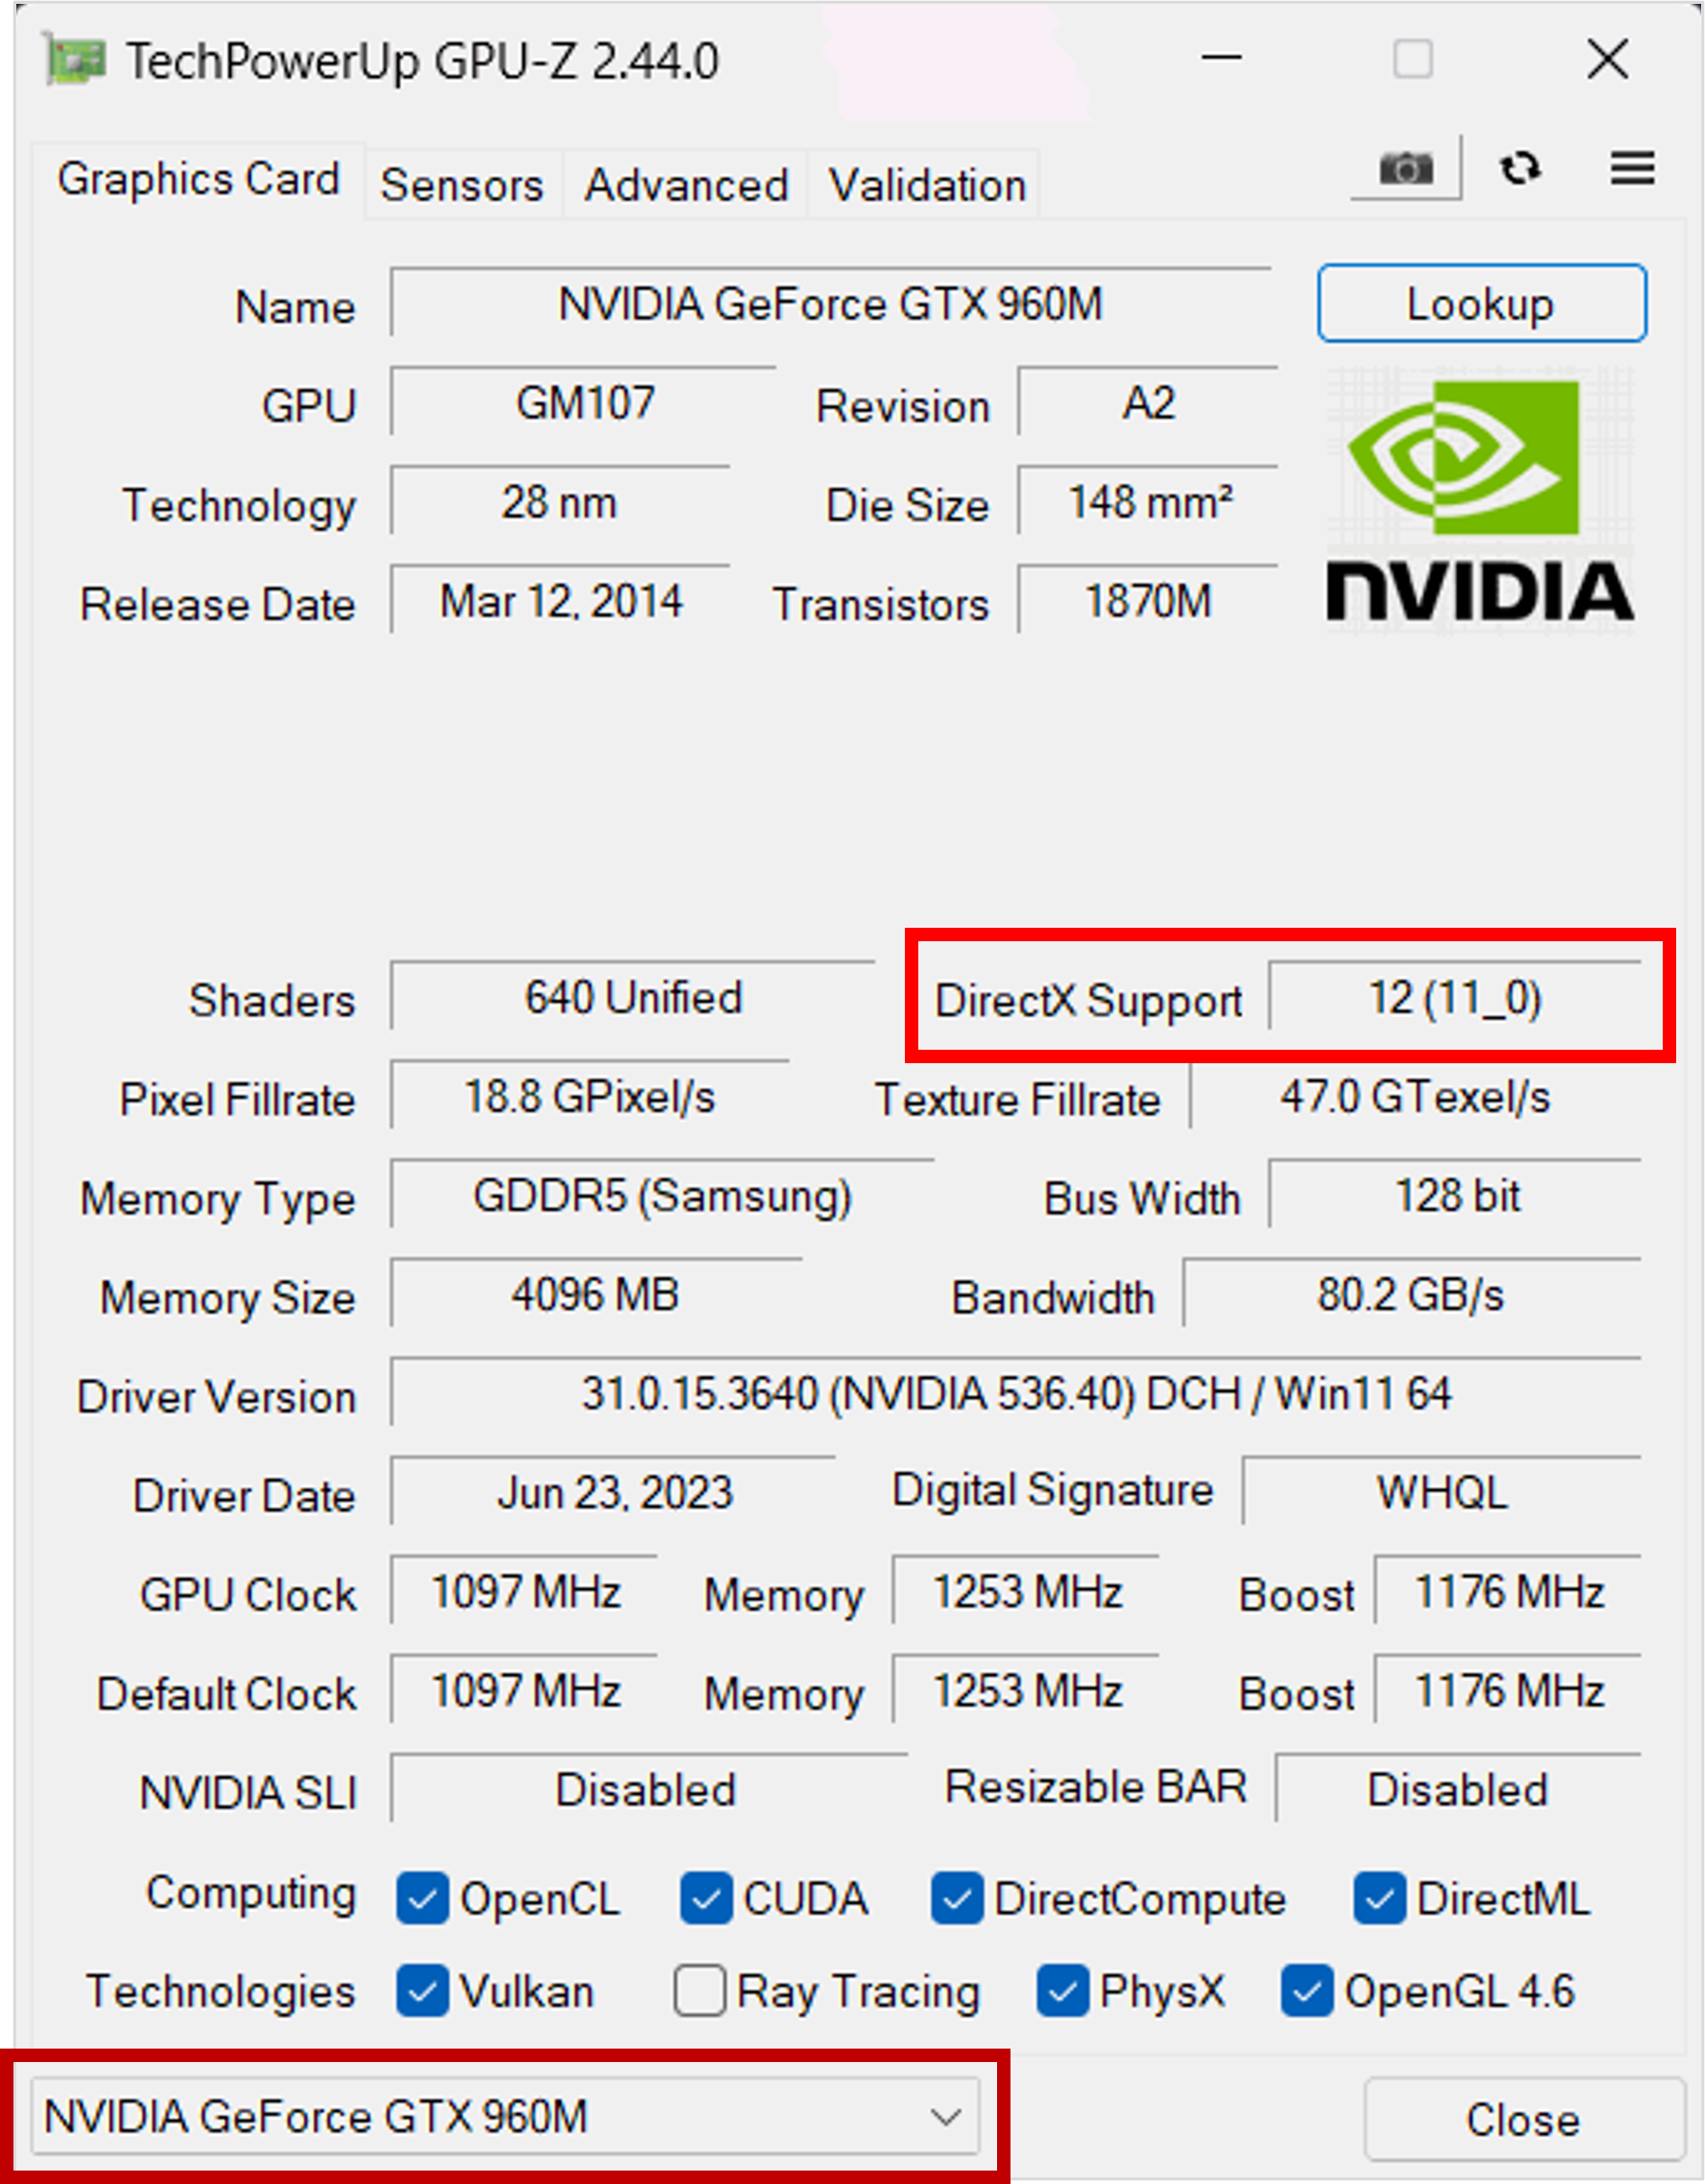
\includegraphics[scale=0.50]{Images/3.Intro.0.1.png}
        \caption*{\Large محیط برنامه ی \lr{GPU-Z} \textbf{\vspace{12pt}}}
    \end{figure}
\end{theo}
\textbf{\vspace{25pt}}

\title{
    \LARGE
    \textbf{استفاده از اسناد \lr{SDK DIRECTX} و نمونه های \lr{SDK}}
} \rullFillWithLine[0.5em]{1pt}
\textbf{\vspace{12pt}}

{
    \Large
    \lr{Direct3D} یک \lr{API} بزرگ است و ما نمی‌توانیم تمام جزئیات آن را در این یک کتاب پوشش دهیم.
    بنابراین، برای به دست آوردن اطلاعات بیشتر، ضروری است نحوه استفاده از اسناد \lr{DirectX SDK} را یاد بگیرید.
    به روزترین اسناد در \lr{\href{https://learn.microsoft.com/en-us/windows/win32/direct3d12/directx-12-programming-guide}{MSDN}} در دسترس خواهند بود.

    \begin{figure}[H]
        \centering
        \setlength{\belowcaptionskip}{-10pt}
        
\includegraphics[scale=0.15]{Images/1.Intro.0.2.png}
                \caption*{\Large \lr{\href{https://learn.microsoft.com/en-us/windows/win32/direct3d12/directx-12-programming-guide}{https://learn.microsoft.com/en-us/windows/win32/direct3d12/directx-12-programming-guide}}}
    \end{figure}

    شکل 1 تصویری از مستندات آنلاین را نشان می‌دهد.
    اسناد \lr{DirectX} تقریباً همه‌ی بخش‌های \lr{DirectX API} را پوشش می‌دهد.
    بنابراین این اسناد می‌تواند یک مرجع بسیار مفید باشد، اما از آنجایی که مستندات آنچنان وارد جزئیات نمی‌شوند، می‌توان گفت که این اسناد بهترین ابزار یادگیری نیستند. با این حال، با هر نسخه جدید \lr{DirectX} که منتشر شود، اسناد نیز بهتر و بهتر می‌شود.

    همانطور که گفته شد، اسناد به عنوان یک مرجع قابل استفاده هستند.
    فرض کنید با یک نوع یا تابع مرتبط با \lr{DirectX} مواجه شده‌اید که اطلاعات بیشتری در مورد آن می‌خواهید، به عنوان مثال تابع \lr{\grayBox{ID3D12Device::CreateCommittedResource}}.
    شما می‌توانید به سادگی در مستندات جستجو کنید و توضیحاتی از نوع آن شی یا در این مثال، توضیحاتی در مورد تابع دریافت کنید. شکل 2 را ببینید.

    \begin{figure}[H]
        \centering
        \setlength{\belowcaptionskip}{-10pt}
        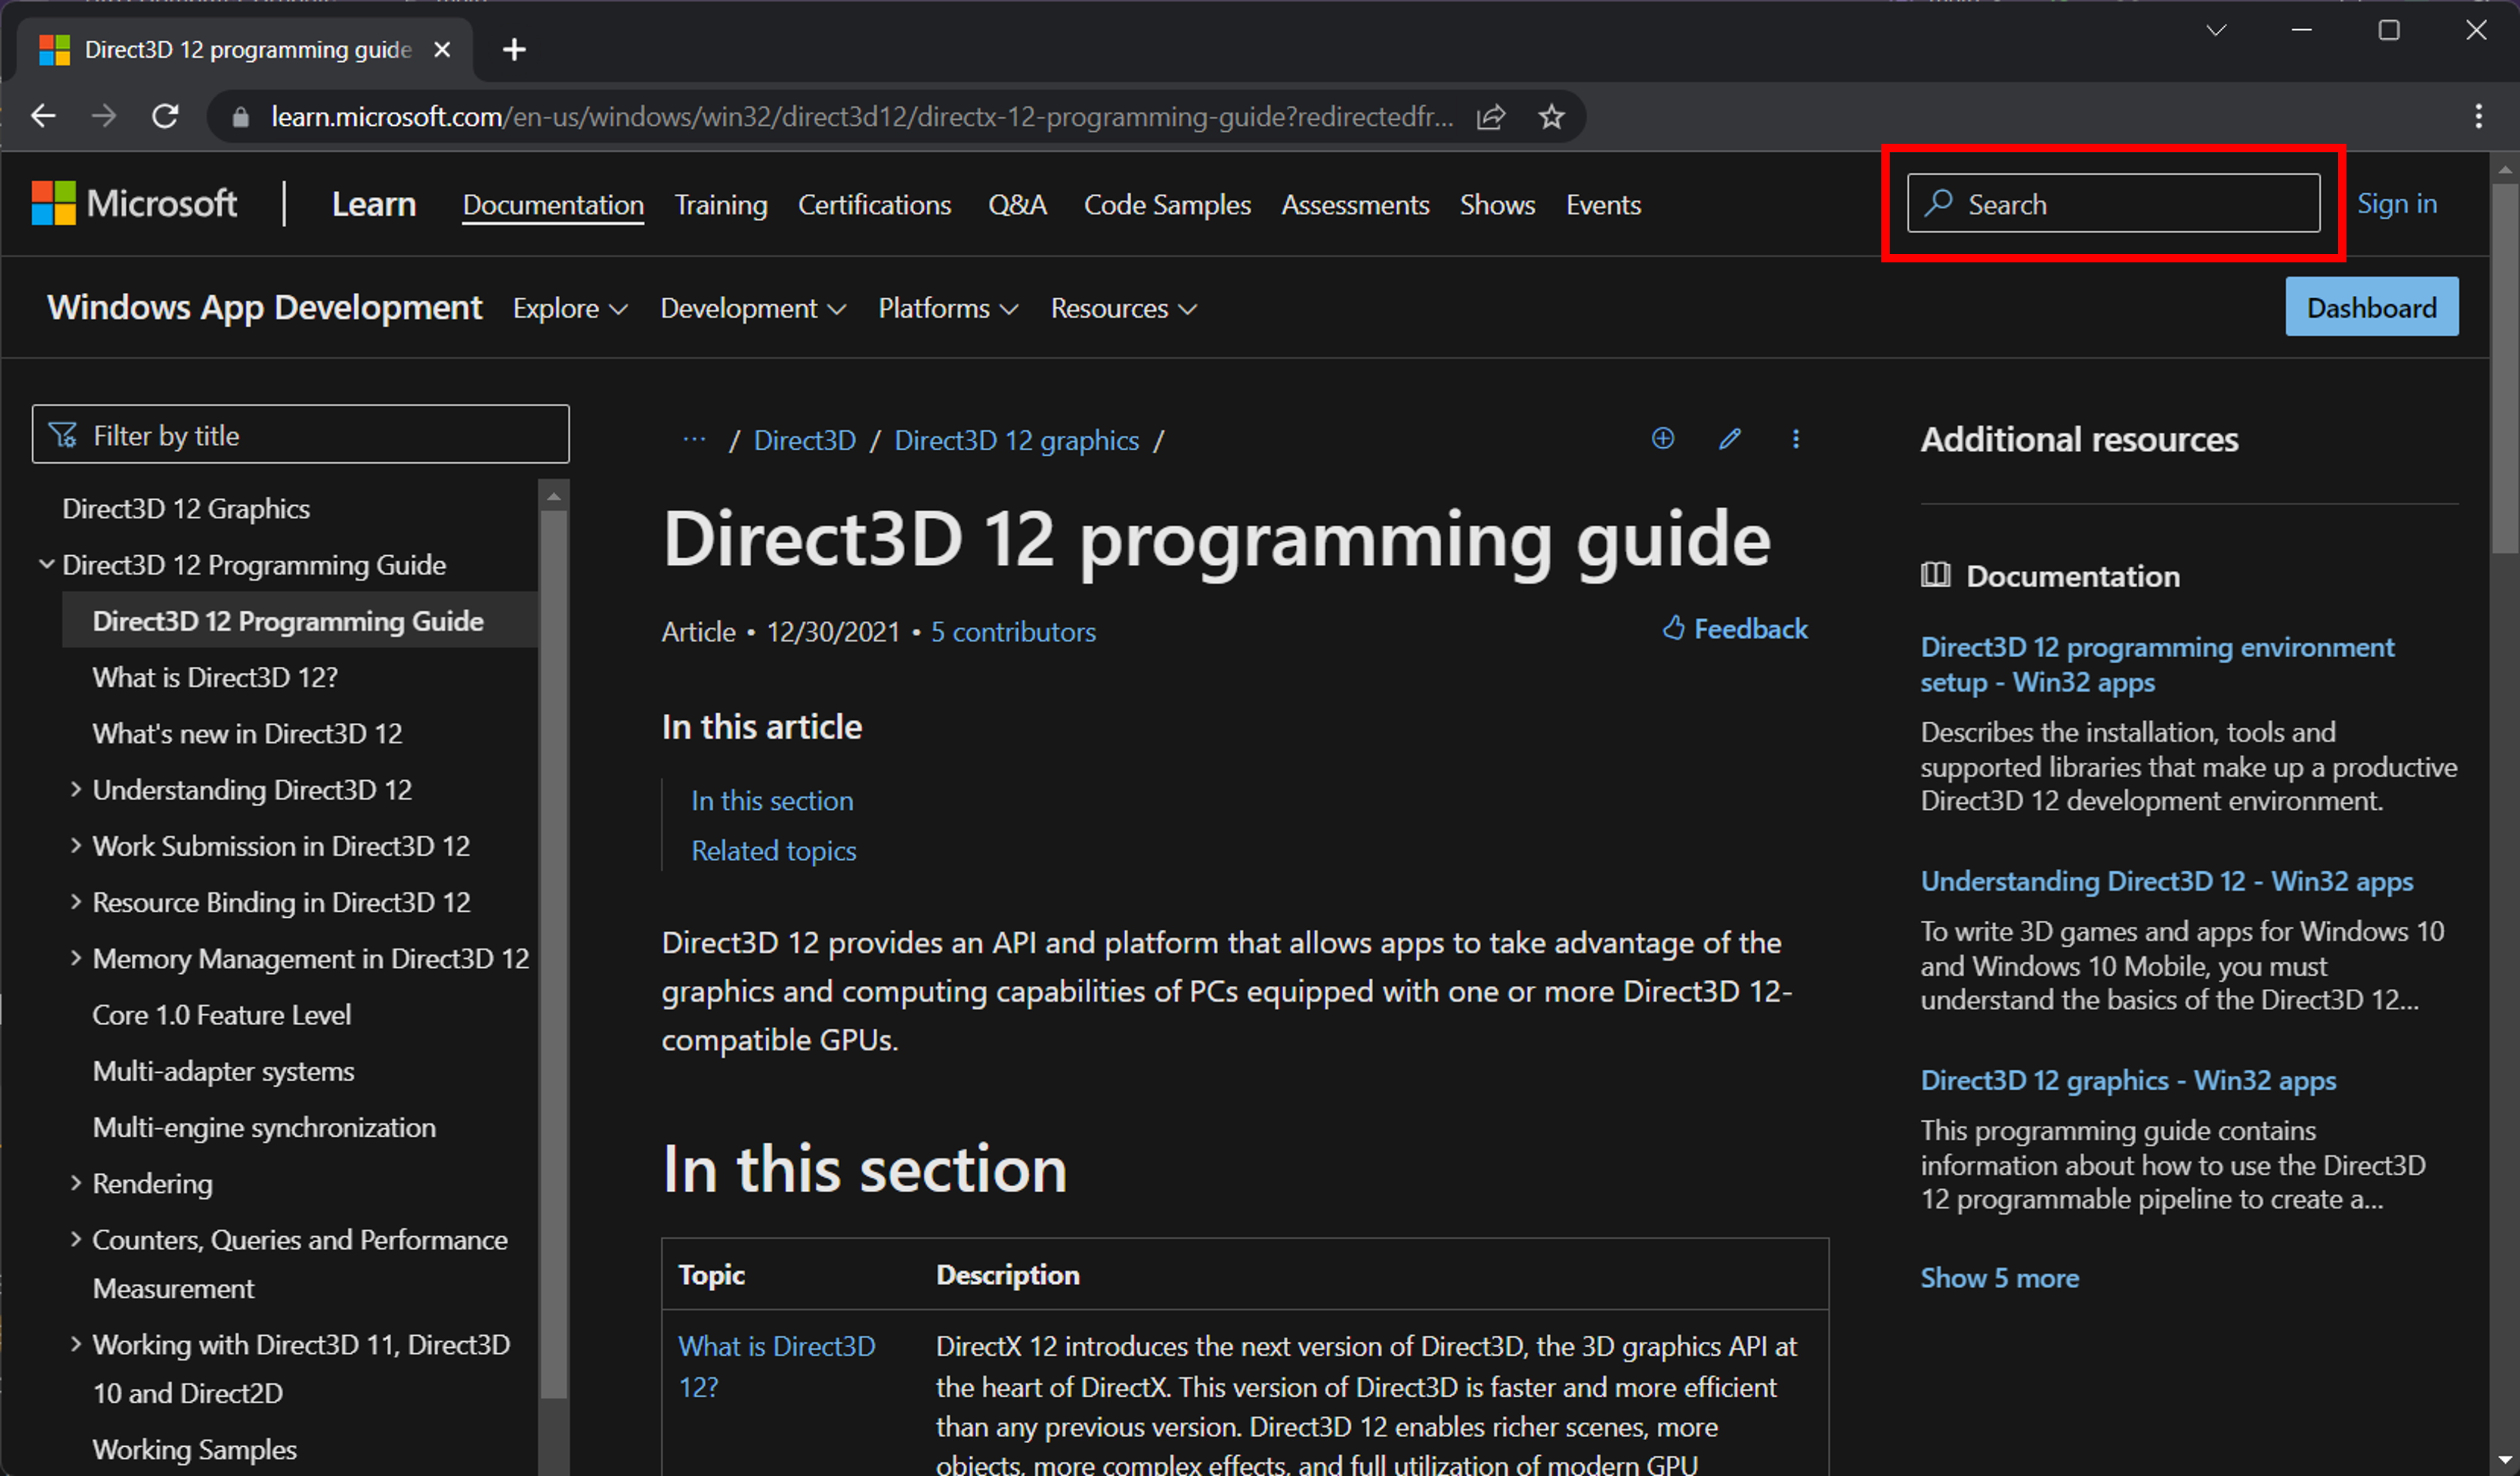
\includegraphics[width=\textwidth]{Images/1.Intro.1.1.png}
        \caption{راهنمای برنامه نویسی \lr{Direct3D} در مستندات \lr{DirectX}}
        \\[20pt]
        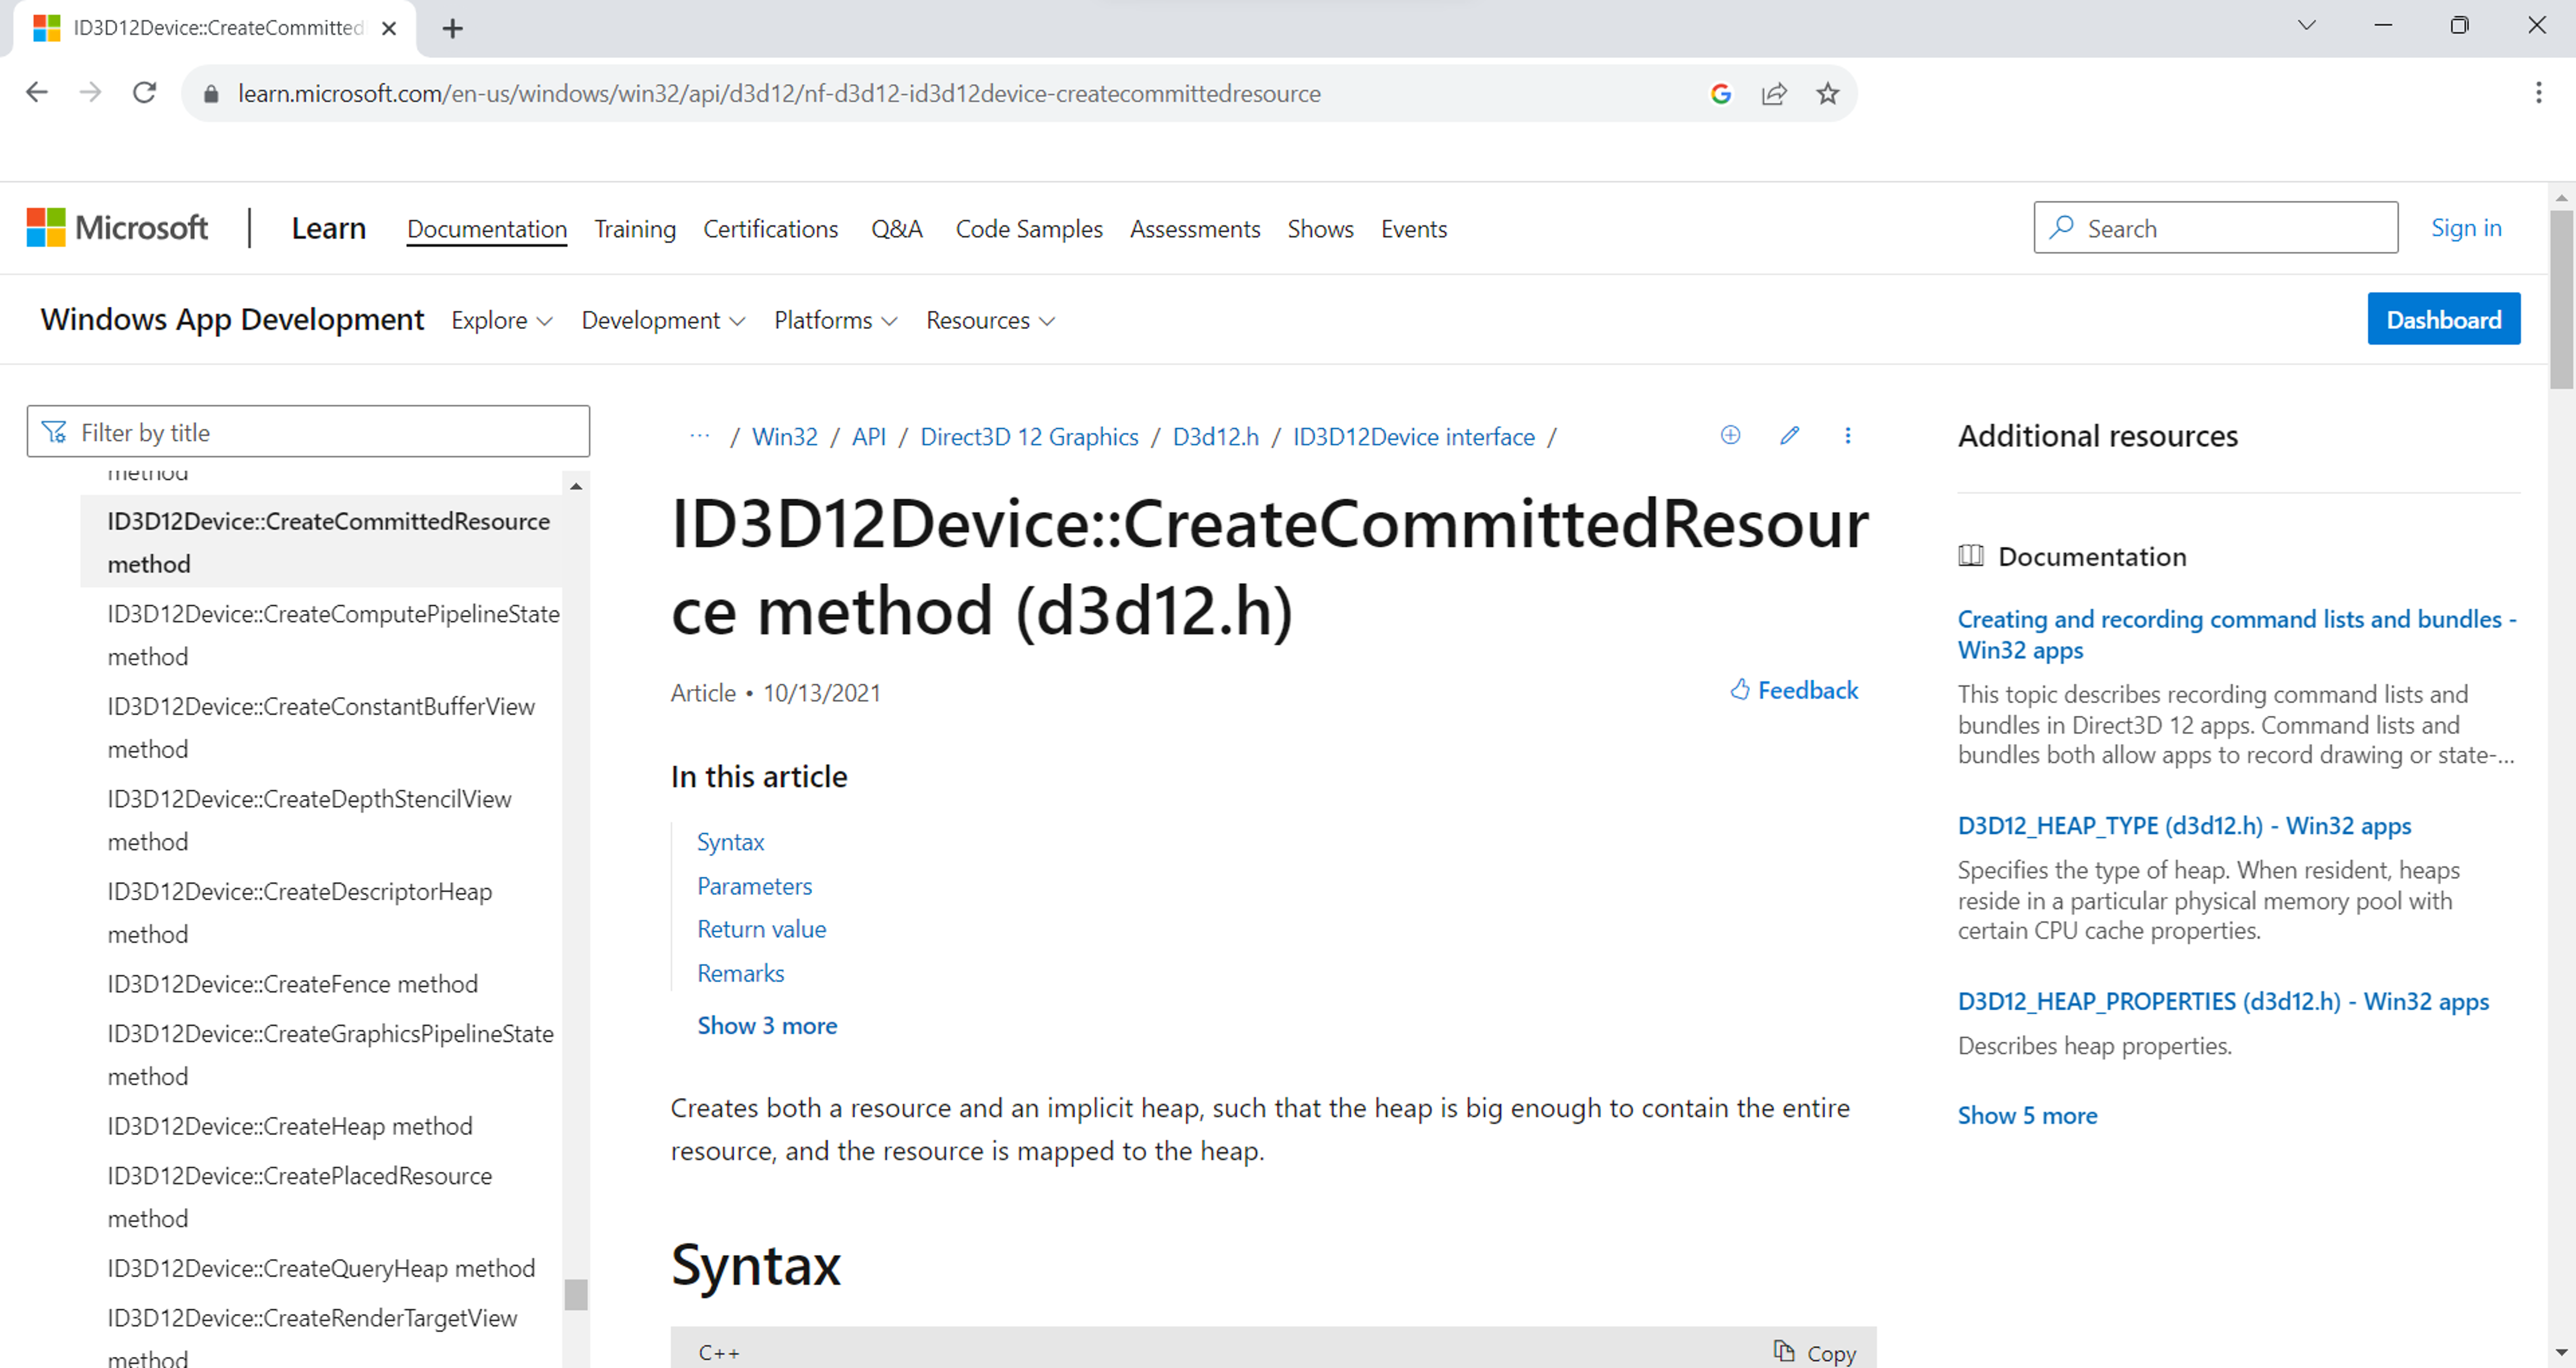
\includegraphics[width=\textwidth]{Images/1.Intro.1.2.png}
        \caption{دریافت مستندات یک تابع}
    \end{figure}

    \begin{theo}{thm:pythagoras}
        در این کتاب ممکن است هر از گاهی برای جزئیات بیشتر شما را به مستندات راهنمایی کنیم.
    \end{theo}
    همچنین برنامه های نمونه \lr{Direct3D 12} که به صورت آنلاین در دسترس هستند را میتوانید در لینک زیر مشاهده کنید:

    \begin{figure}[H]
        \centering
        \setlength{\belowcaptionskip}{-10pt}
        
\includegraphics[scale=0.15]{Images/1.Intro.0.2.png}
        \caption*{\Large \lr{\href{https://github.com/Microsoft/DirectX-Graphics-Samples}{https://github.com/Microsoft/DirectX-Graphics-Samples}}}
    \end{figure}

    میتوانید نمونه‌های \lr{Direct3D 12} را در وب‌سایت‌های \lr{NVIDIA}، \lr{AMD} و \lr{Intel} مشاهده کنید. همچنین در آینده نمونه‌های بیشتری نیز خواهند آمد.
}
\textbf{\vspace{25pt}}

\title{
    \LARGE
    \textbf{شفاف سازی}
} \rullFillWithLine[0.5em]{1pt}
\textbf{\vspace{12pt}}

{
    \Large
    اگرچه ما تلاش می‌کنیم که کد‌های کارآمدی بنویسیم و همزمان از بهترین شیوه‌های برنامه‌نویسی \lr{Direct3D 12} استفاده کنیم، اما هدف اصلی هر برنامه‌ی نمونه، نشان دادن مفاهیم \lr{Direct3D} یا تکنیک‌های برنامه‌نویسی گرافیکی است.
    هدف ما نوشتن بهینه‌ترین کد نیست زیرا به احتمال زیاد، این کار‌ایده‌هایی را که تلاش می‌کردیم به تصویر بکشیم را مبهم می‌کرد.
    اگر از کد نمونه در پروژه‌های خود استفاده می‌کنید، این نکته را در نظر داشته باشید، زیرا باید برای کارایی بهتر دوباره روی آن کار کنید.
    علاوه بر این، به منظور تمرکز بر \lr{Direct3D API}، زیرساخت‌های حداقلی را در بالای \lr{Direct3D} ایجاد کرده‌ایم. به این معنی که ما مقادیر را هاردکد (\lr{hardcode}) کردیم و چیز‌هایی را در کد منبع تعریف کردیم که ممکن است مبتنی بر داده باشند.
در یک برنامه بزرگ سه بعدی، احتمالاً یک موتور رندرینگ در بالای \lr{Direct3D} پیاده‌سازی خواهید کرد. با این حال، موضوع این کتاب \lr{Direct3D API} است، نه طراحی موتور‌های رندرینگ.
}
\textbf{\vspace{25pt}}

\title{
    \LARGE
    \textbf{نمونه برنامه ها و مکمل های آنلاین}
} \rullFillWithLine[0.5em]{1pt}
\textbf{\vspace{12pt}}

{
    \Large
    وب‌سایت‌های این کتاب (\href{www.d3dcoder.net}{www.d3dcoder.net} و \href{www.merclearning.com}{www.merclearning.com}) نقش مهمی در استفاده حداکثری از این کتاب دارد. [\textbf{مترجم:} همه‌ی لینک‌ها و منابع در سایت من به صورت یکجا وجود دارند و نیازی نیست تمامی لینک‌های کتاب را ذخیره یا باز کنید. ]
    در وب سایت شما کد منبع کامل و فایل‌های پروژه برای هر نمونه در این کتاب را خواهید یافت.
    در بسیاری از موارد، برنامه‌های \lr{DirectX} آنقدر بزرگ هستند که نمی‌توانند به طور کامل در یک کتاب متنی جاسازی شوند. بنابراین، ما فقط قطعات کد مربوطه را بر اساس‌ایده‌هایی که نشان داده می‌شوند نشان می‌دهیم.
    اکیداً توصیه می‌شود که خواننده کد آزمایشی مربوطه را مطالعه کند تا برنامه را به طور کامل ببیند (هدف ما این است که آزمایشی‌ها (\lr{demos}) را برای مطالعه آسان کوچک و متمرکز کنیم). به عنوان یک قاعده کلی، خواننده باید بتواند پس از خواندن فصل و گذراندن مدتی برای مطالعه کد نسخه‌ی آزمایشی، کد نسخه (ها)ی آزمایشی فصل را به تنهایی پیاده‌سازی کند.
در واقع اینکه سعی کنید نمونه‌ها را خودتان با استفاده از کتاب و کد نمونه (به عنوان مرجع) پیاده‌سازی کنید، یک تمرین بسیار خوب است.
}
\textbf{\vspace{25pt}}

\title{
    \LARGE
    \textbf{راه اندازی پروژه آزمایشی در \lr{Visual Studio 2022}}
} \rullFillWithLine[0.5em]{1pt}
\textbf{\vspace{12pt}}

{
    \Large
    آزمایشی‌های این کتاب را می‌توانید به سادگی با دوبار کلیک کردن روی فایل پروژه مربوطه \lr{(.vcxproj)} یا فایل \lr{solution (.sln)} باز کنید.
    این بخش نحوه‌ی باز کردن یا ایجاد و ساخت یک پروژه را از ابتدا با استفاده از چارچوب برنامه آزمایشی کتاب با استفاده از \lr{Visual Studio 2022} توضیح می‌دهد.
    به عنوان یک مثال کاربردی، نحوه بازآفرینی و build کردن نسخه آزمایشی \lr{\"Box\"} از فصل 6 را نشان خواهیم داد.
}
\textbf{\vspace{25pt}}

\title{
    \Large
    \rullCenterTextWithLine{\textbf{کد منبع کتاب را دانلود کنید}}
}

{
    \Large
    ابتدا کد منبع کتاب را در پوشه‌ای در هارد دیسک خود دانلود کنید.
    فرض می‌کنیم این پوشه \grayBox{\lr{C:\symbol{92}d3d12book}} است.
    در پوشه کد منبع، فهرستی از پوشه‌ها از هر فصل را خواهید دید. هر پوشه شامل پروژه‌های کد برای فصل داده شده است.
    همچنین به پوشه‌ای به نام \lr{Common} توجه کنید. این پوشه حاوی کد منبع به اشتراک گذاشته شده است که در تمام پروژه‌های آزمایشی استفاده مجدد می‌شود.
    اکنون، در پوشه کد منبع، یک پوشه جدید ایجاد کنید که می‌خواهید آزمایشی‌های خود را در آن ذخیره کنید.
    برای مثال، \grayBox{\lr{C:\symbol{92}d3d12book\symbol{92}MyDemos}}. این پوشه جایی است که می‌توانید پروژه‌های جدید را بر اساس چارچوب نمونه‌ی کتاب ایجاد کنید.
}
{
    \Large
    این ساختار پوشه‌بندی ضروری نیست، اما ساختاری است که آزمایشی‌های کتاب از آن پیروی می‌کنند. اگر با تنظیم مسیر‌های اضافی راحت هستید، می‌توانید پروژه‌های آزمایشی خود را در هر مکانی قرار دهید و \lr{Visual Studio} را تنظیم کنید که کد منبع را در دایرکتوری \lr{Common} پیدا کند.
}
\textbf{\vspace{25pt}}

\title{
    \Large
    \rullCenterTextWithLine{\textbf{موارد مورد نیاز \lr{Visual Studio} را نصب کنید}}
}

{
    \Large
    در صورتی که \lr{Visual Studio} را نصب نکرده‌اید، ابتدا آن را با استفاده از راهنما‌های آنلاین نصب کنید. پس از نصب آن، ابتدا \lr{Visual Studio Installer} را باز کنید. از پنجره‌ی باز شده، \lr{Modify} یا \lr{Install} را کلیک کنید. در سمت چپ پنجره‌ی باز شده، از قسمت \lr{\grayBox{Desktop \& Mobile}}، تیک قسمت‌های \lr{Universal Windows Platform development} و \lr{Desktop development with C++} را در صورتی که انتخاب نشده‌اند، بزنید.
از قسمت \lr{\grayBox{Gaming}} نیز تیک \lr{Game development with C++} را بزنید.

    \begin{figure}[H]
        \centering
        \setlength{\belowcaptionskip}{-10pt}
        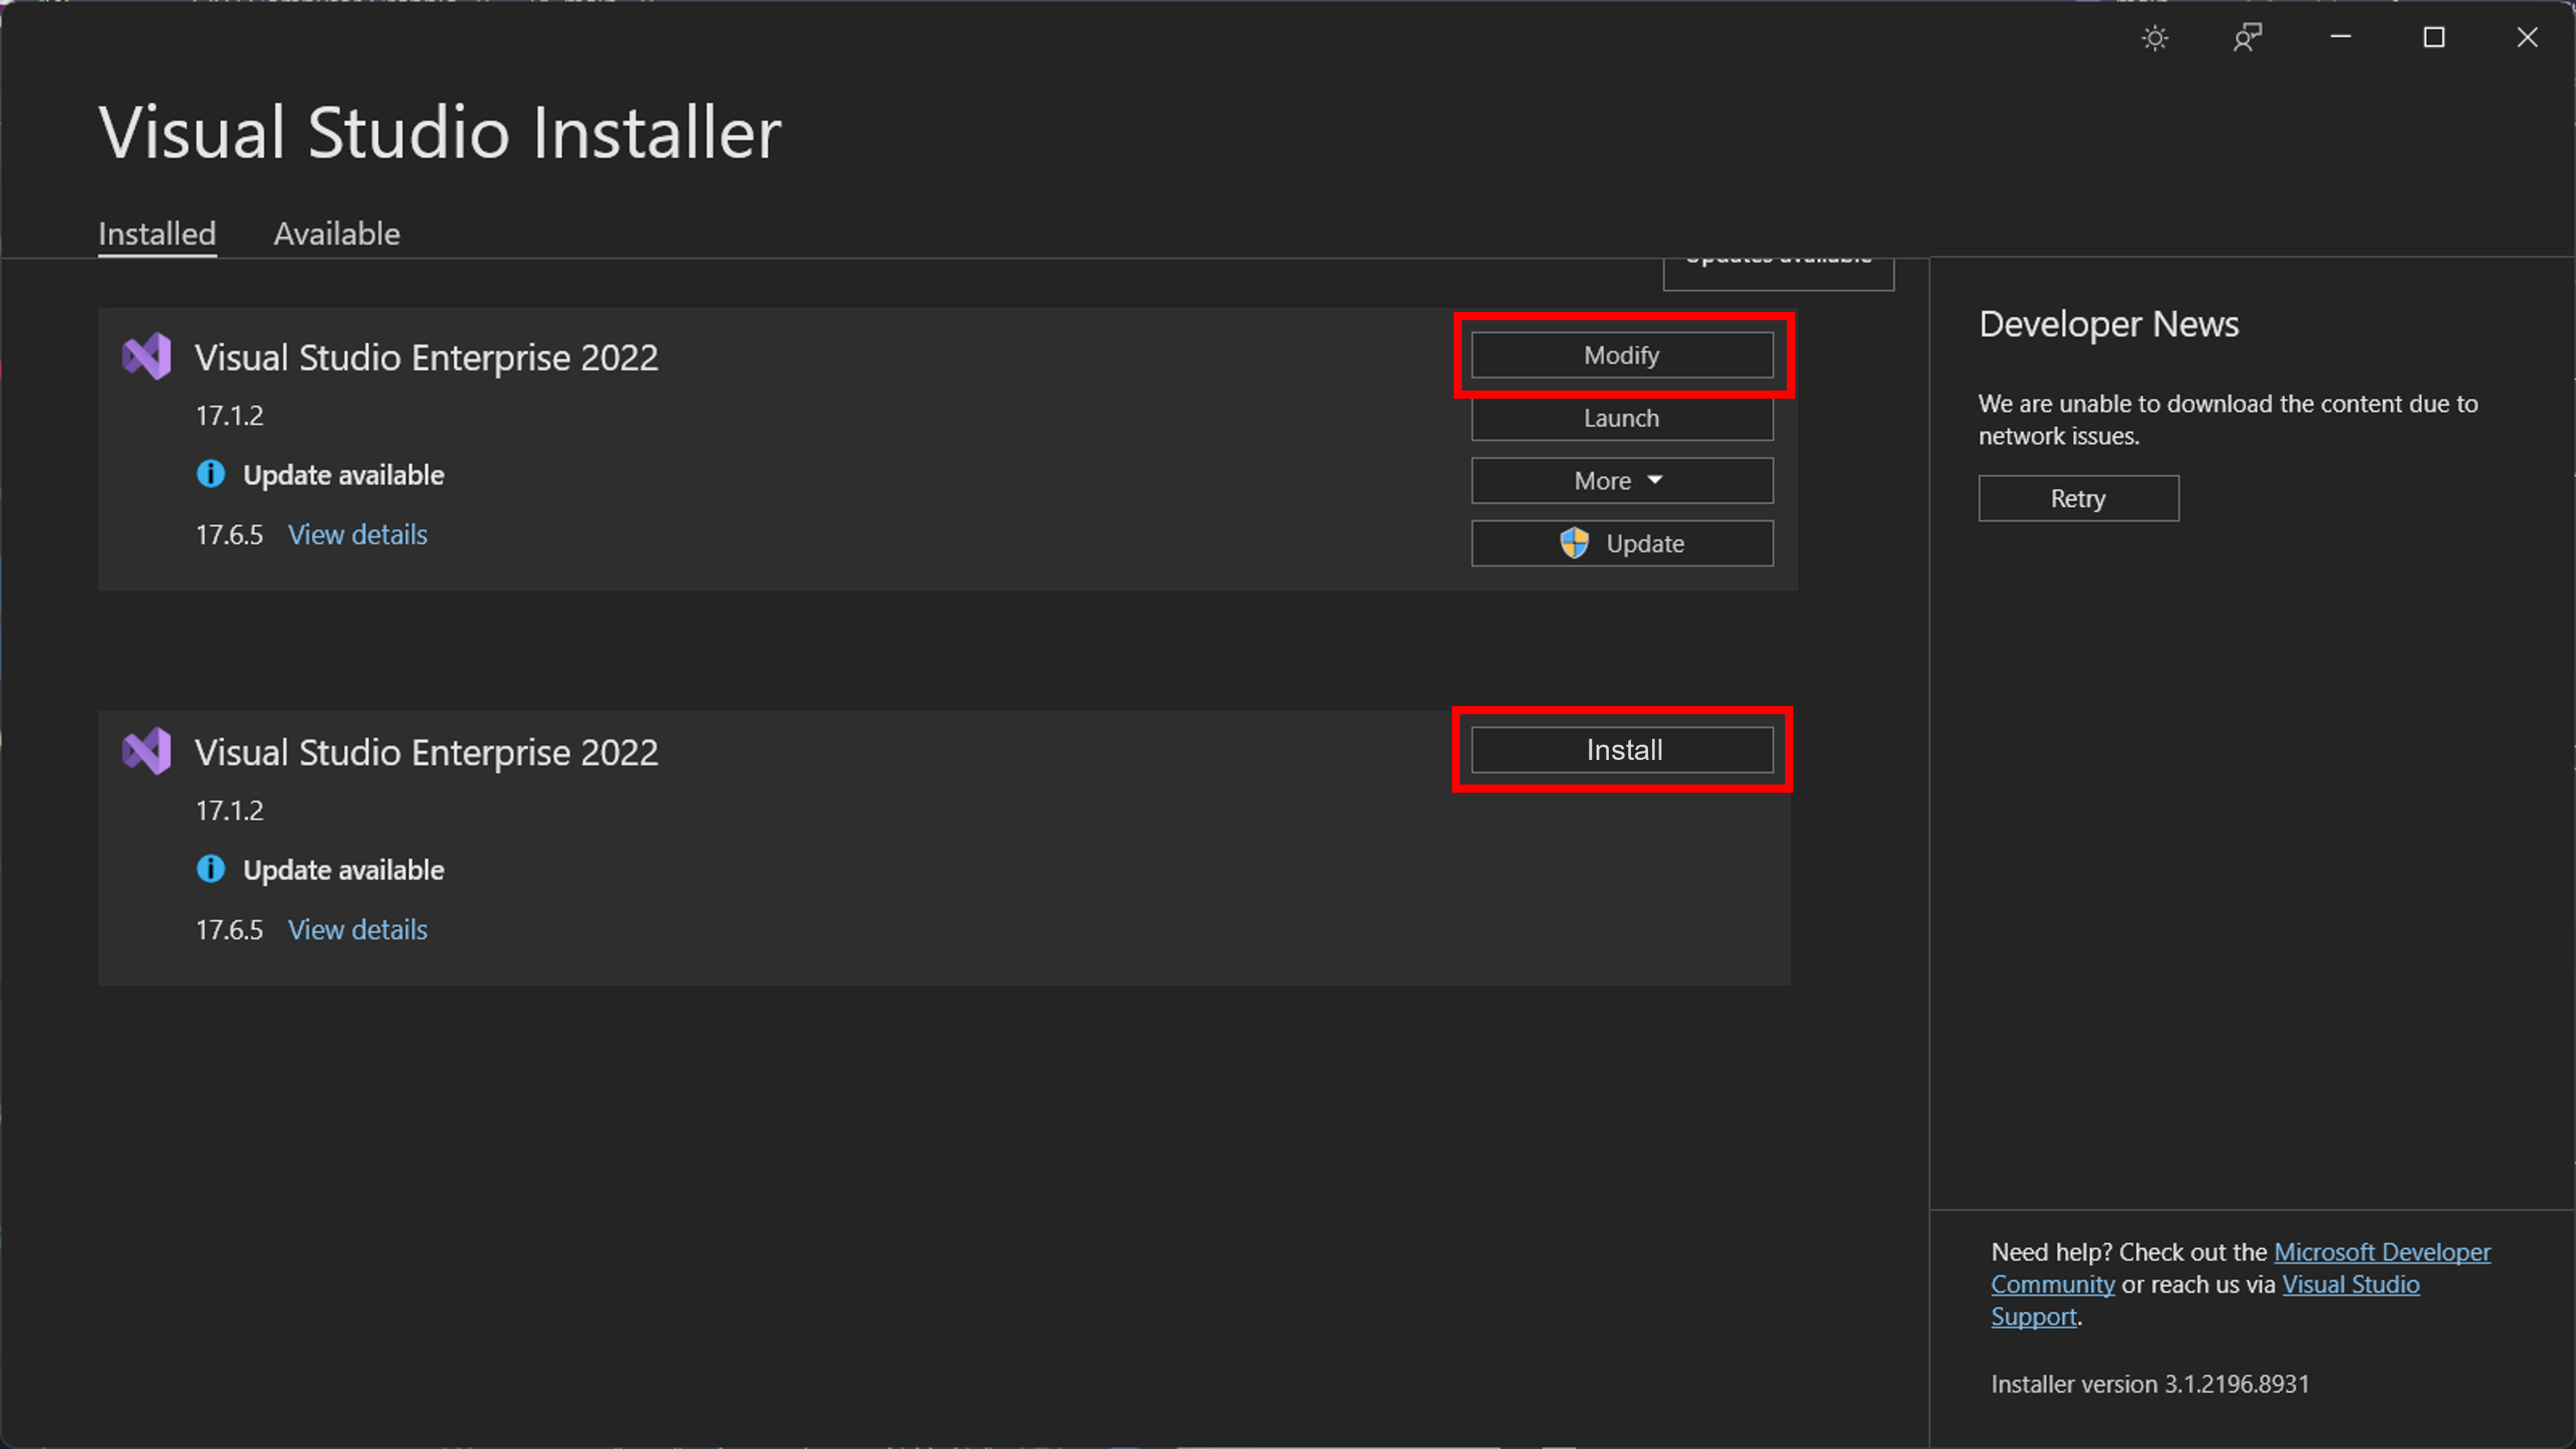
\includegraphics[width=\textwidth]{Images/1.Intro.2.1.png}
        \caption*{محیط \lr{Visual Studio Installer}}
        \\[20pt]
        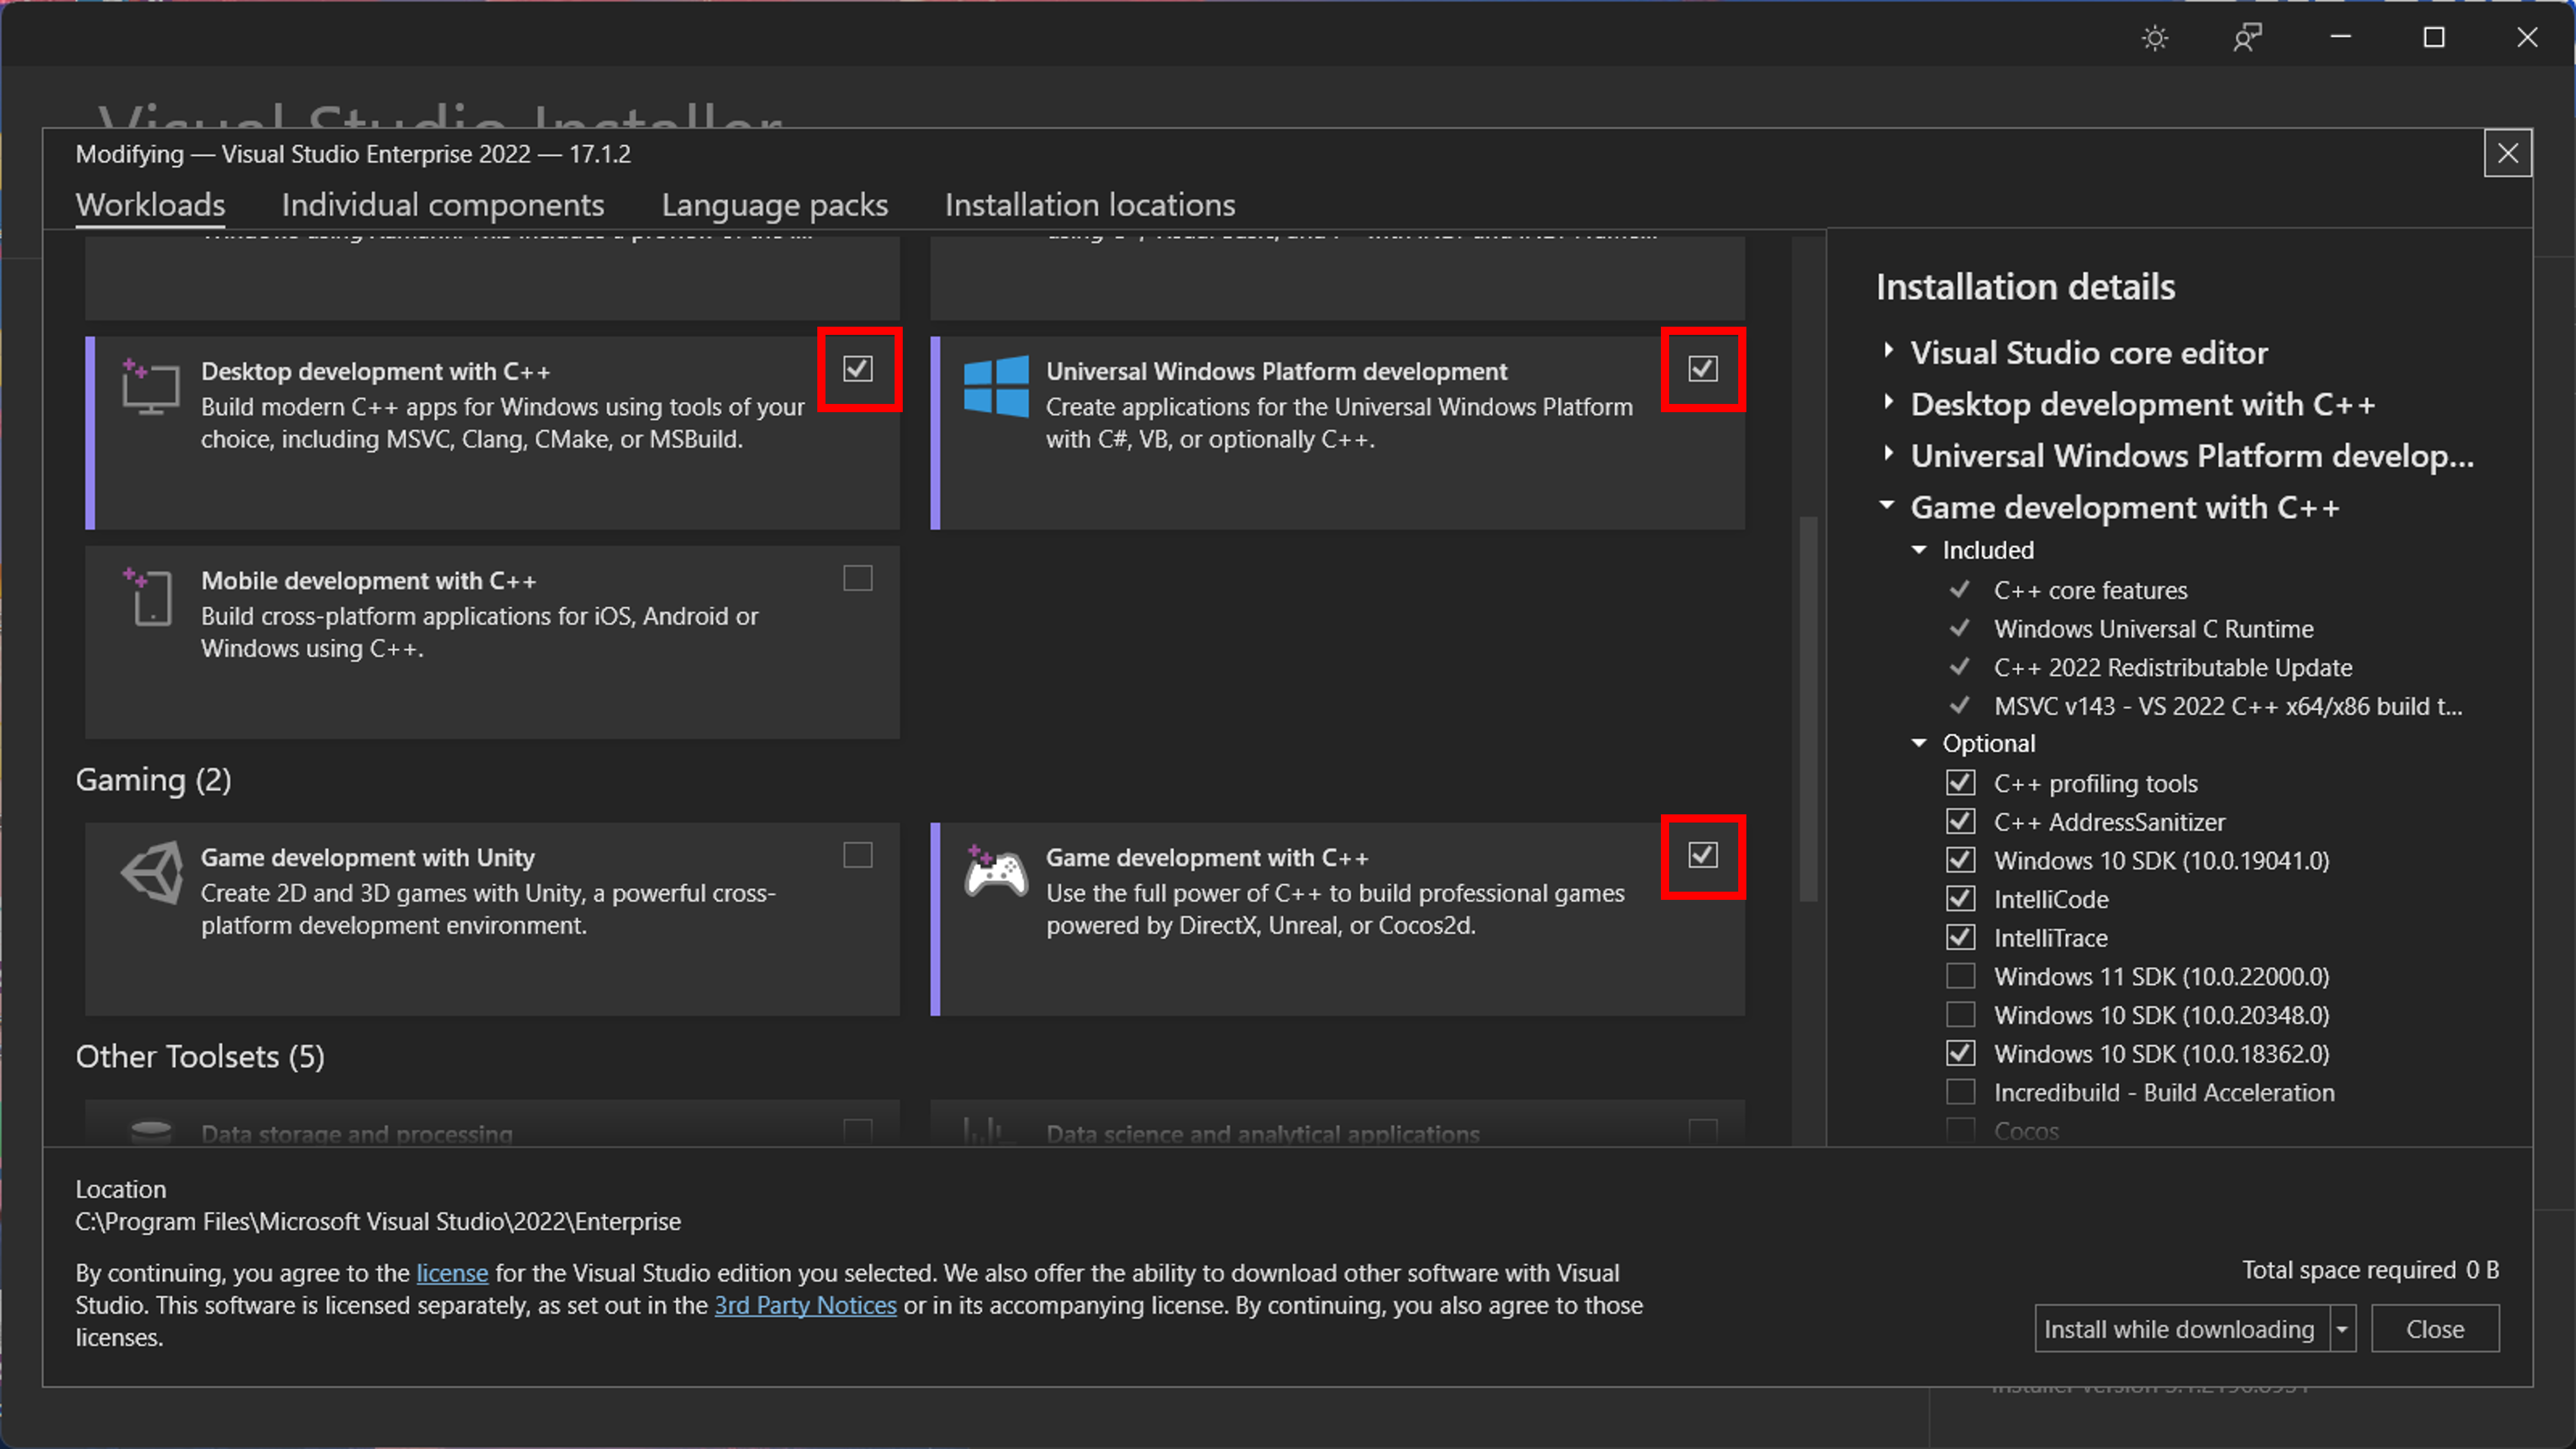
\includegraphics[width=\textwidth]{Images/1.Intro.2.2.png}
        \caption*{مواردی که باید نصب شوند}
    \end{figure}


    بعد از انتخاب موارد بالا، باید موارد اضافه‌تری را نیز انتخاب کنید. این موارد شامل \lr{SDK}‌های ویندوز و ورژن‌های جدید \lr{C++} است.
    در سمت راست پنجره‌ی باز شده، می‌توانید این موارد را ببینید. برای اجرای بهتر، سعی کنید موارد را مانند عکس‌ها رعایت کنید. پس از آن در پایین پنجره روی گزینه‌ی \lr{Install} کلیک کنید تا موارد انتخاب شده نصب شوند.
    \begin{figure}[H]
        \centering
        \setlength{\belowcaptionskip}{-10pt}
        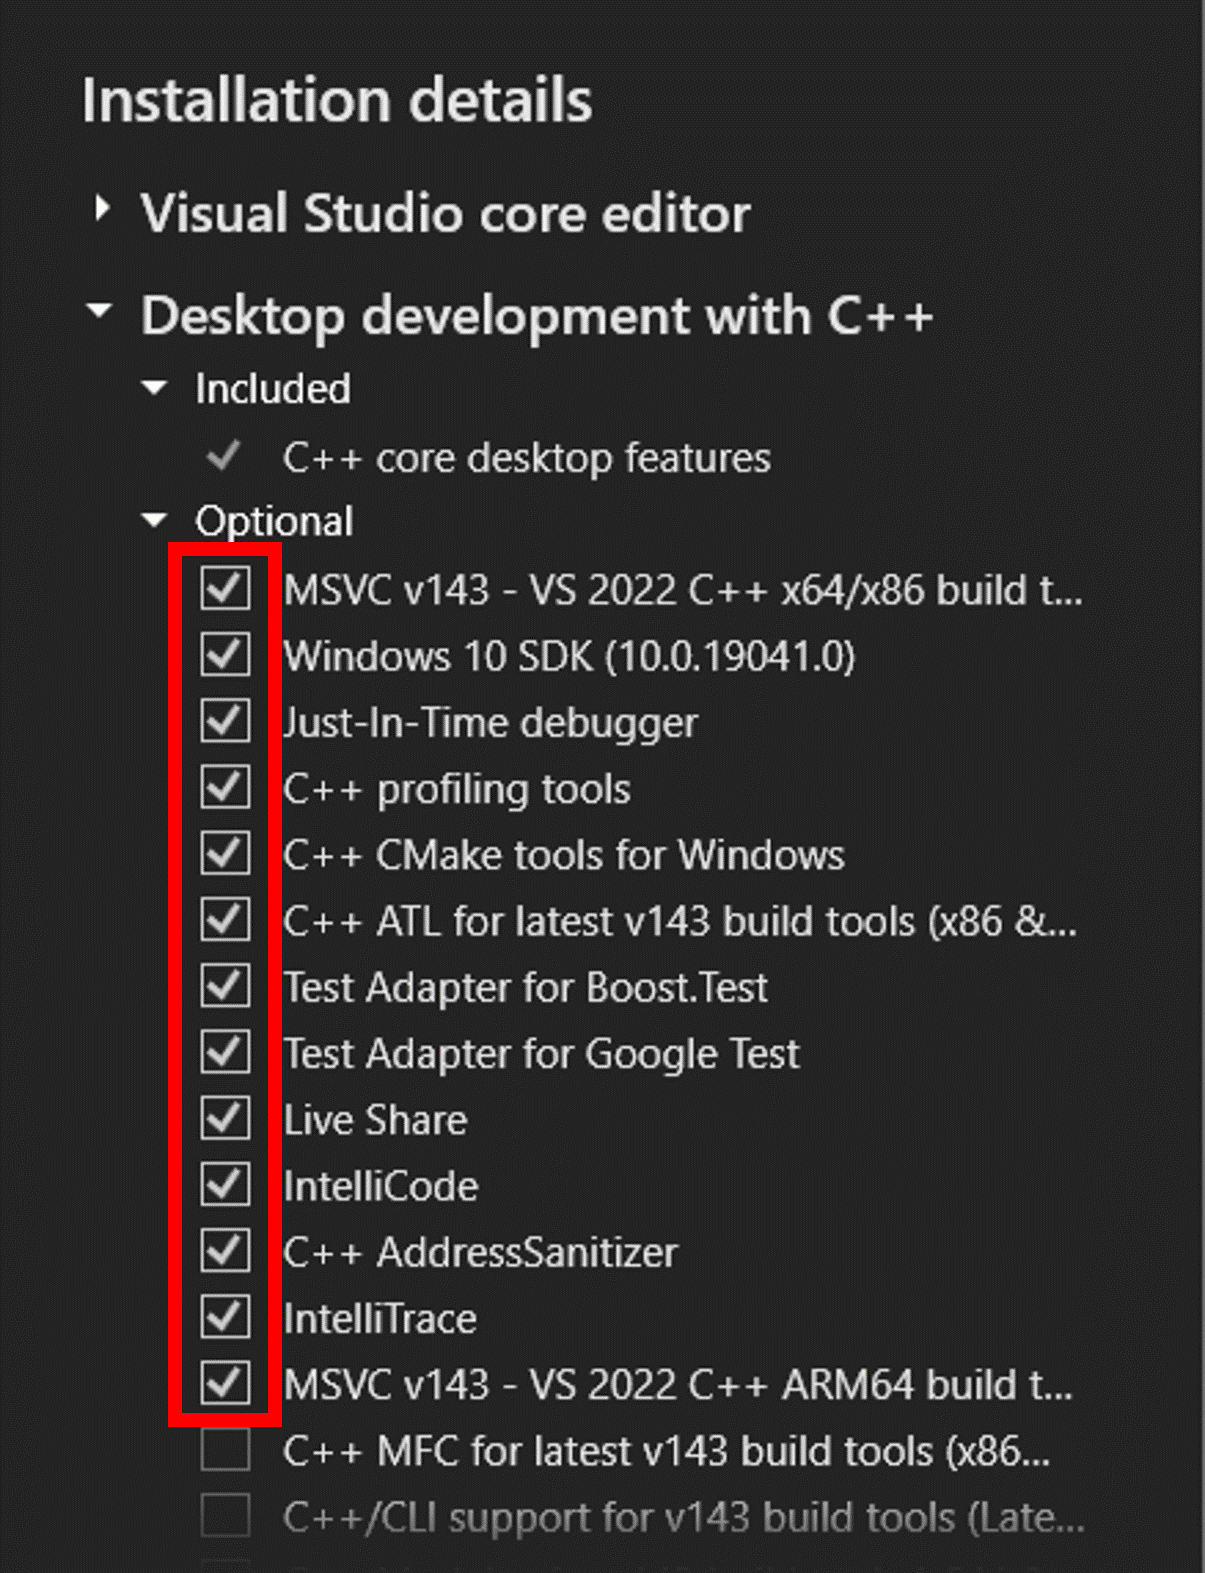
\includegraphics[scale=0.7]{Images/1.Intro.3.1.png} \hspace{5mm}
        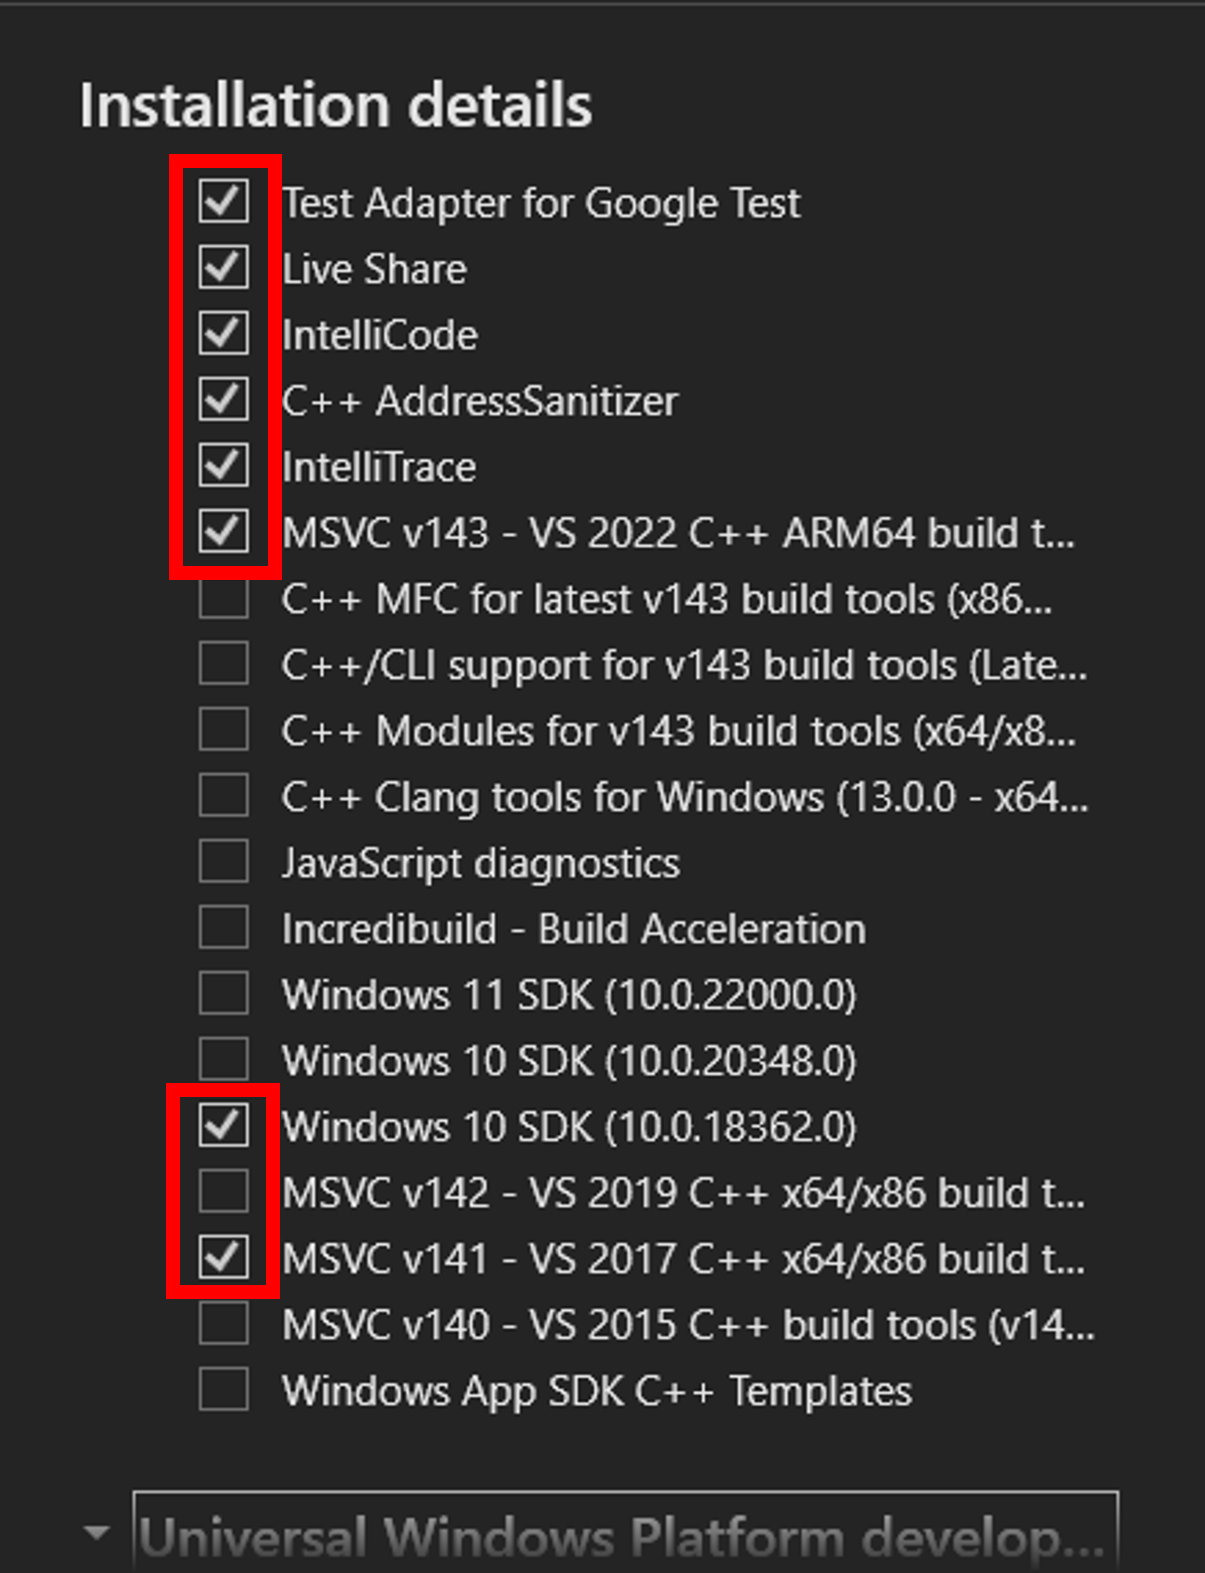
\includegraphics[scale=0.7]{Images/1.Intro.3.2.png}
        \\[25pt]
        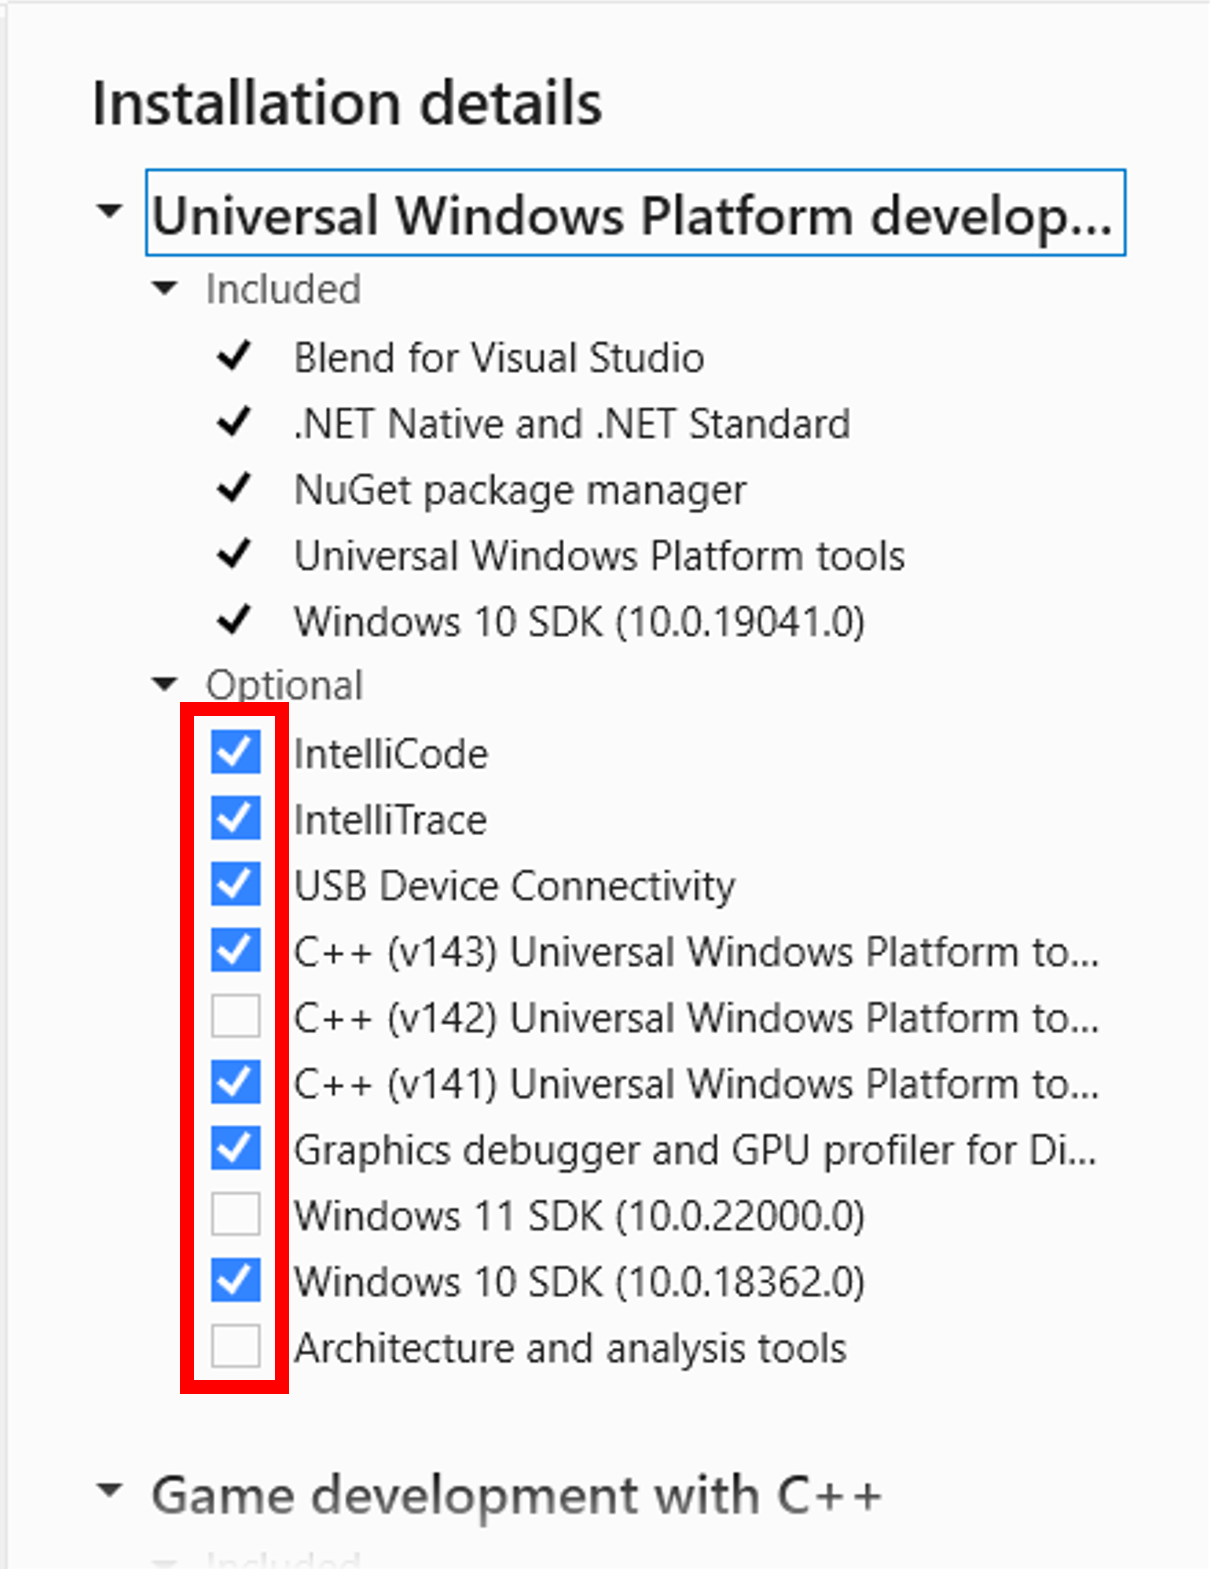
\includegraphics[scale=0.7]{Images/1.Intro.3.3.png} \hspace{5mm}
        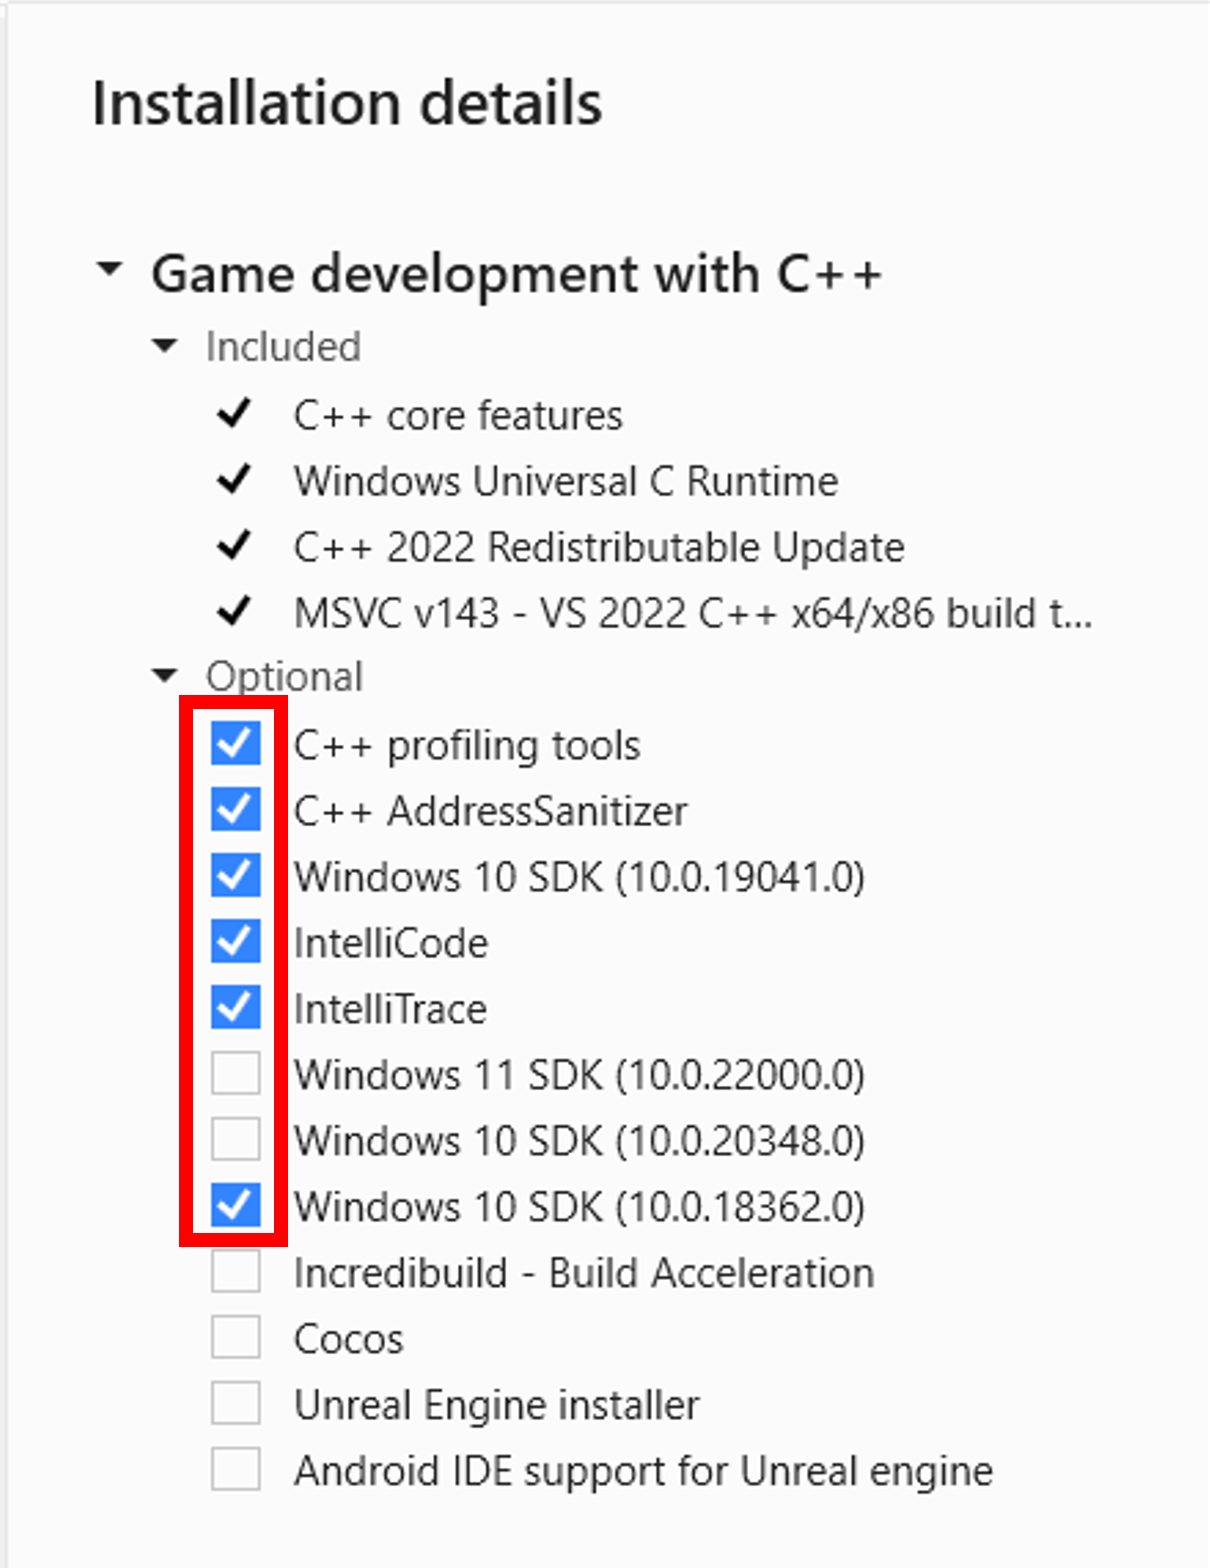
\includegraphics[scale=0.7]{Images/1.Intro.3.4.png}
        \caption*{مواردی که باید نصب شوند.}
    \end{figure}
}
\textbf{\vspace{12pt}}

\title{
    \Large
    \rullCenterTextWithLine{\textbf{فعال کردن \lr{Graphic Tools}}}
}

{
    \Large
    برای اجرای درست برنامه‌های آزمایشی \lr{DirectX 12}، نیاز است که قابلیت \lr{Graphic Tools} در ویندوز شما فعال باشد.
    برای این کار می‌توانید به دو صورت عمل کنید:

    \textbf{روش اول)}
    ابتدا در منوی استارت، \lr{Optional features} را سرچ کرده و آن را باز کنید.
    اگر \lr{Graphic Tools} از قبل بر روی دستگاه شما نصب شده باشد، می‌توانید از قسمت پایین پنجره آن را مشاهده کنید (کادر زرد رنگ)
    در غیر این صورت بر روی \lr{\grayBox{View features}} کلیک کرده و نام آن را سرچ کرده و نصب کنید.

    \begin{figure}[H]
        \centering
        \setlength{\belowcaptionskip}{-10pt}
        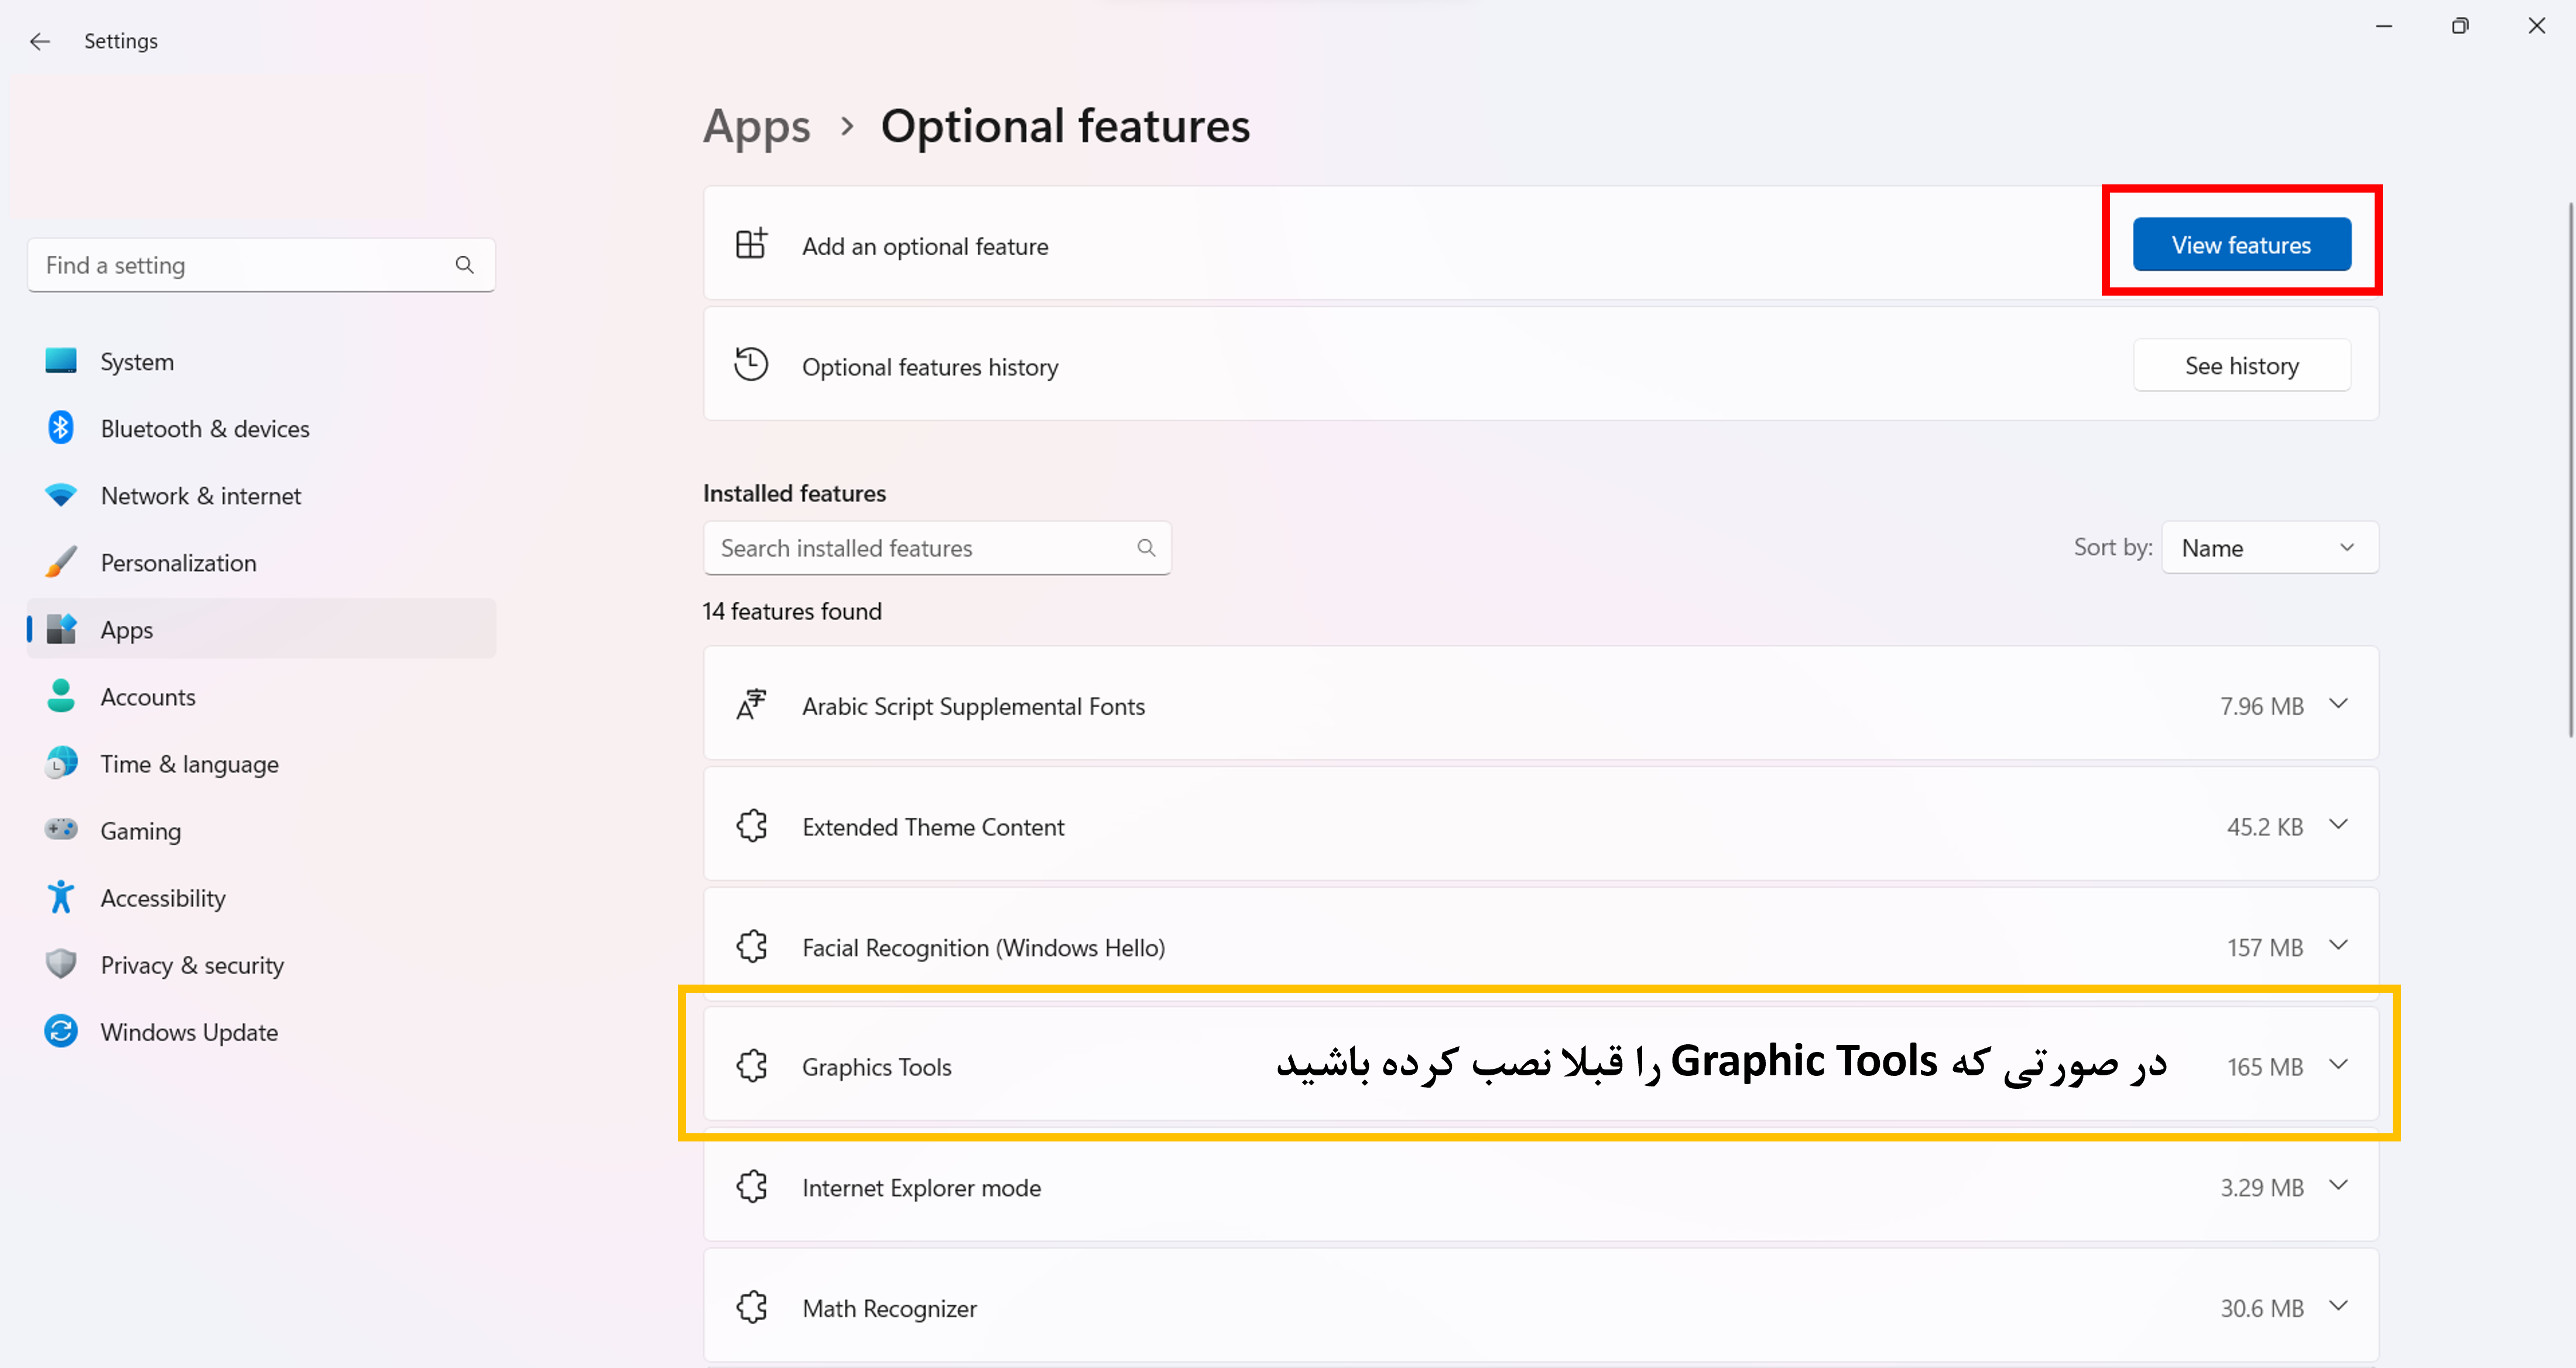
\includegraphics[width=\textwidth]{Images/1.Intro.4.1.png}
        \caption*{محیط \lr{Optional features}}
        \\[25pt]
        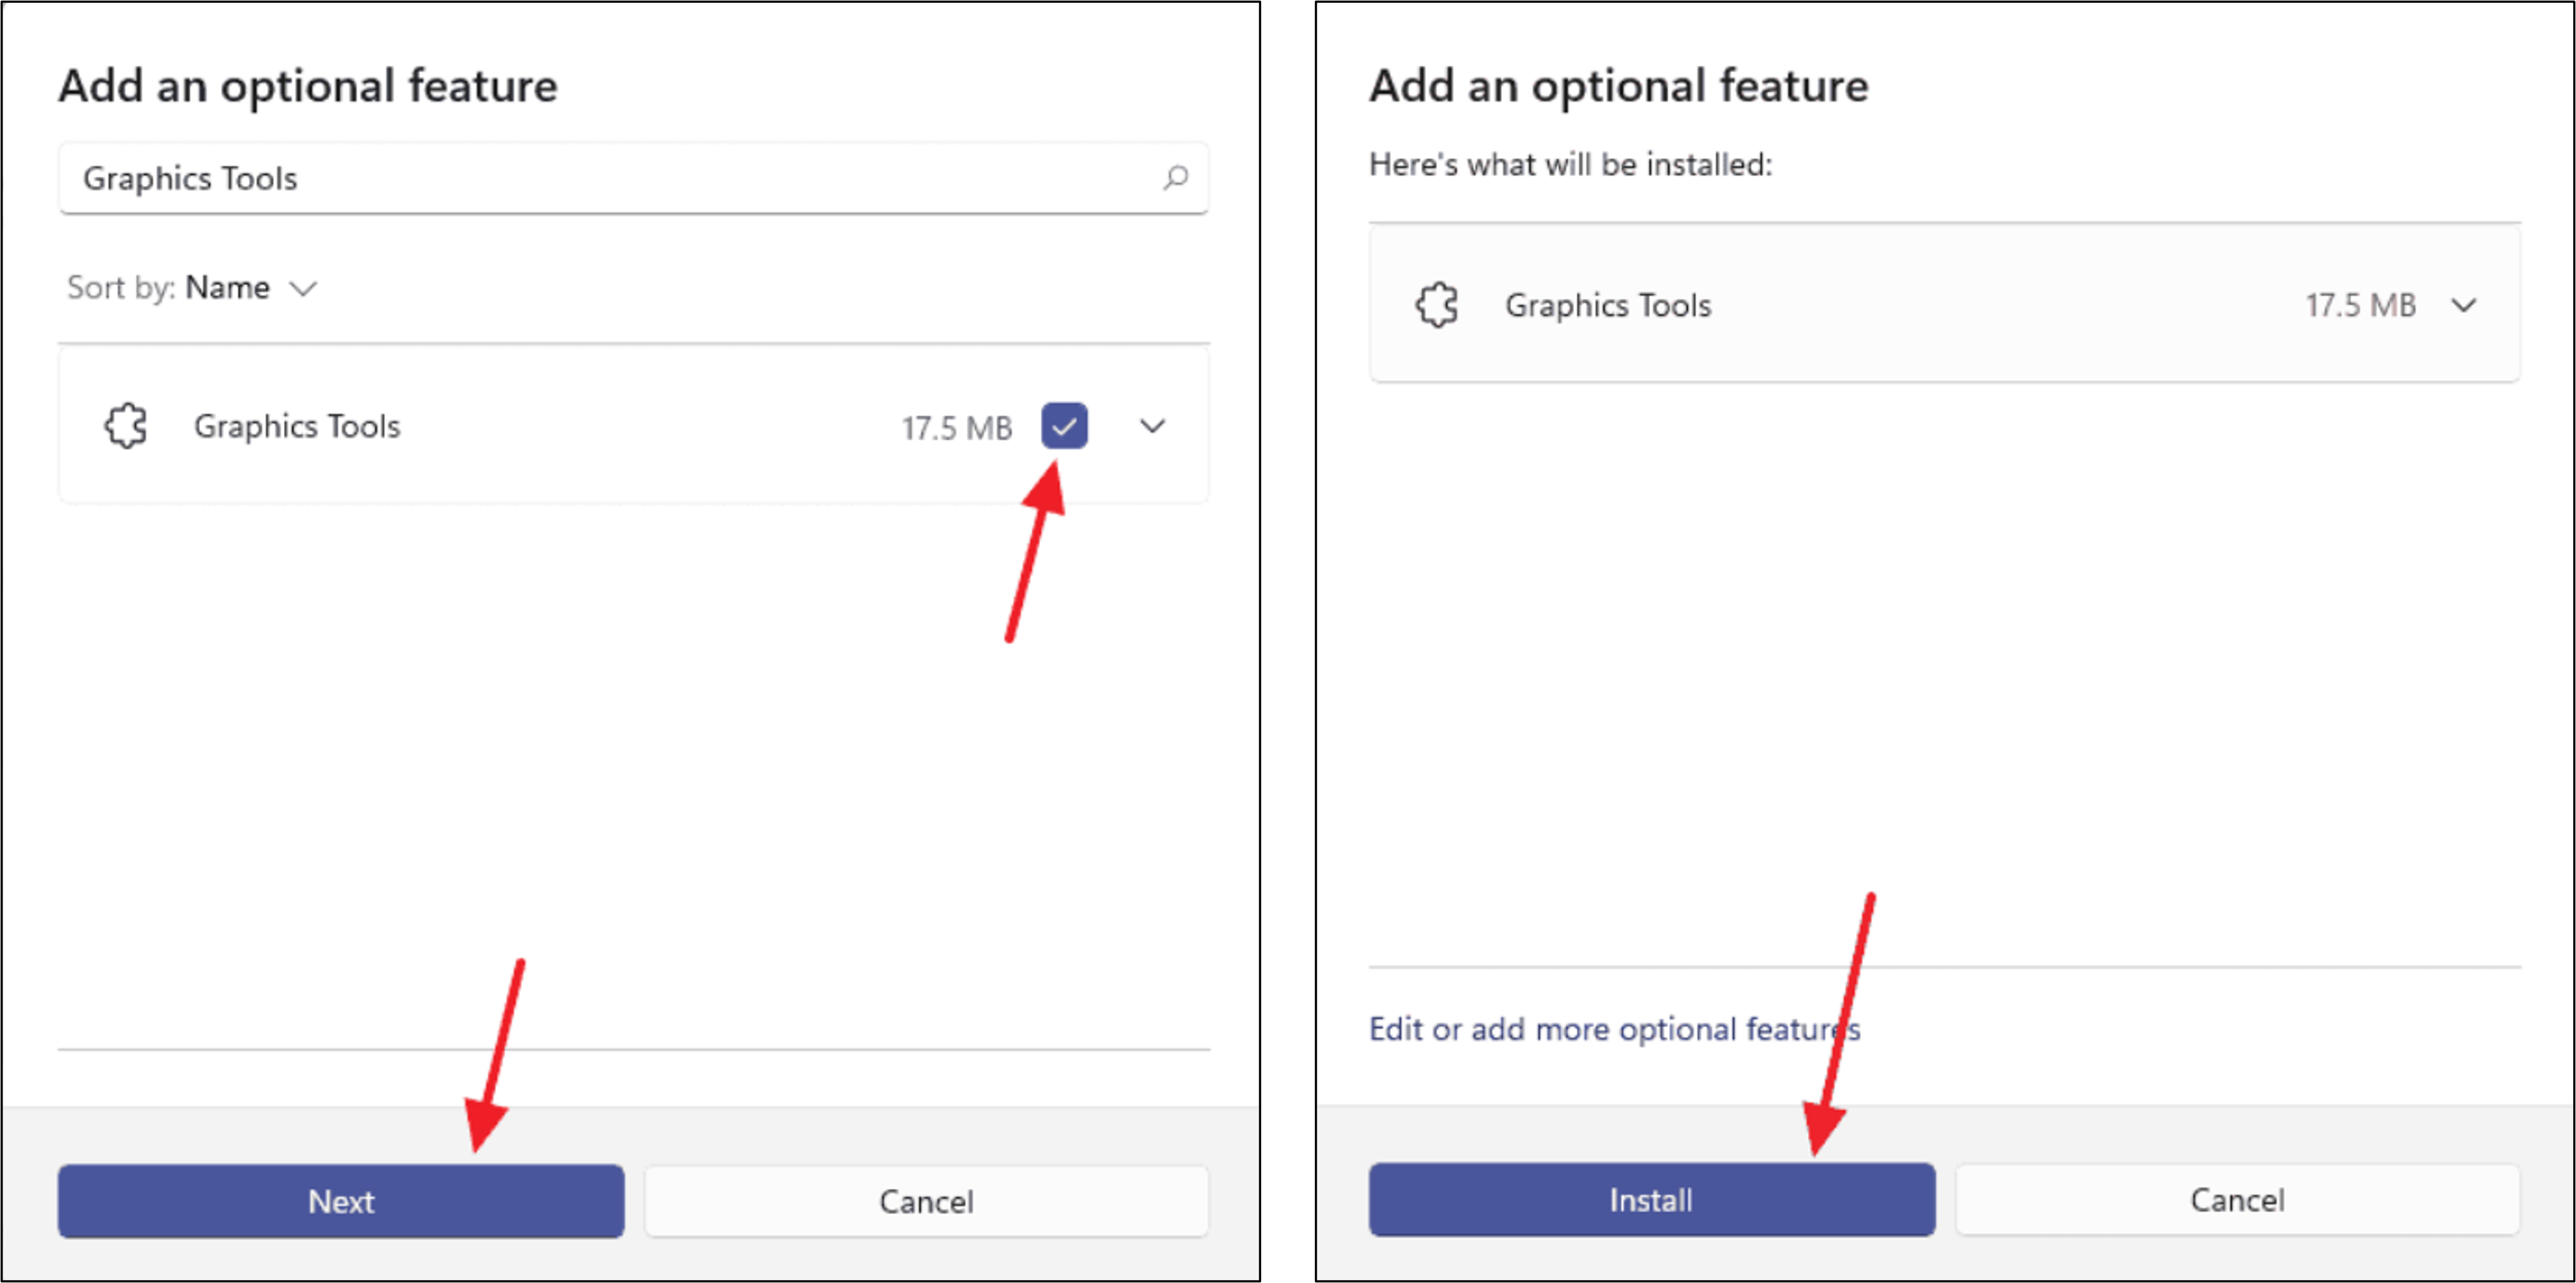
\includegraphics[width=\textwidth]{Images/1.Intro.4.2.png}
        \caption*{نصب \lr{Graphic Tools}}
    \end{figure}

    \textbf{روش دوم)}
    اگر به هر دلیلی روش اول برای شما قابل انجام نبود، می‌توانید پنجره‌ی \lr{Command Prompt} (\lr{CMD}) را به صورت \lr{Run as administrator} باز کرده و با دستورات زیر آن را نصب کنید.

ابتدا دستور داخل \lr{CMD} عبارت زیر را وارد کنید:

    \begin{flushleft}
        \grayBox{\lr{Dism /Online /Get-Packages /Format:Table}}
    \end{flushleft}

    یا با دستور زیر:

    \begin{flushleft}
        \grayBox{\lr{dism /online /Get-Capabilities}}
    \end{flushleft}

    \begin{figure}[H]
        \centering
        \setlength{\belowcaptionskip}{-10pt}
        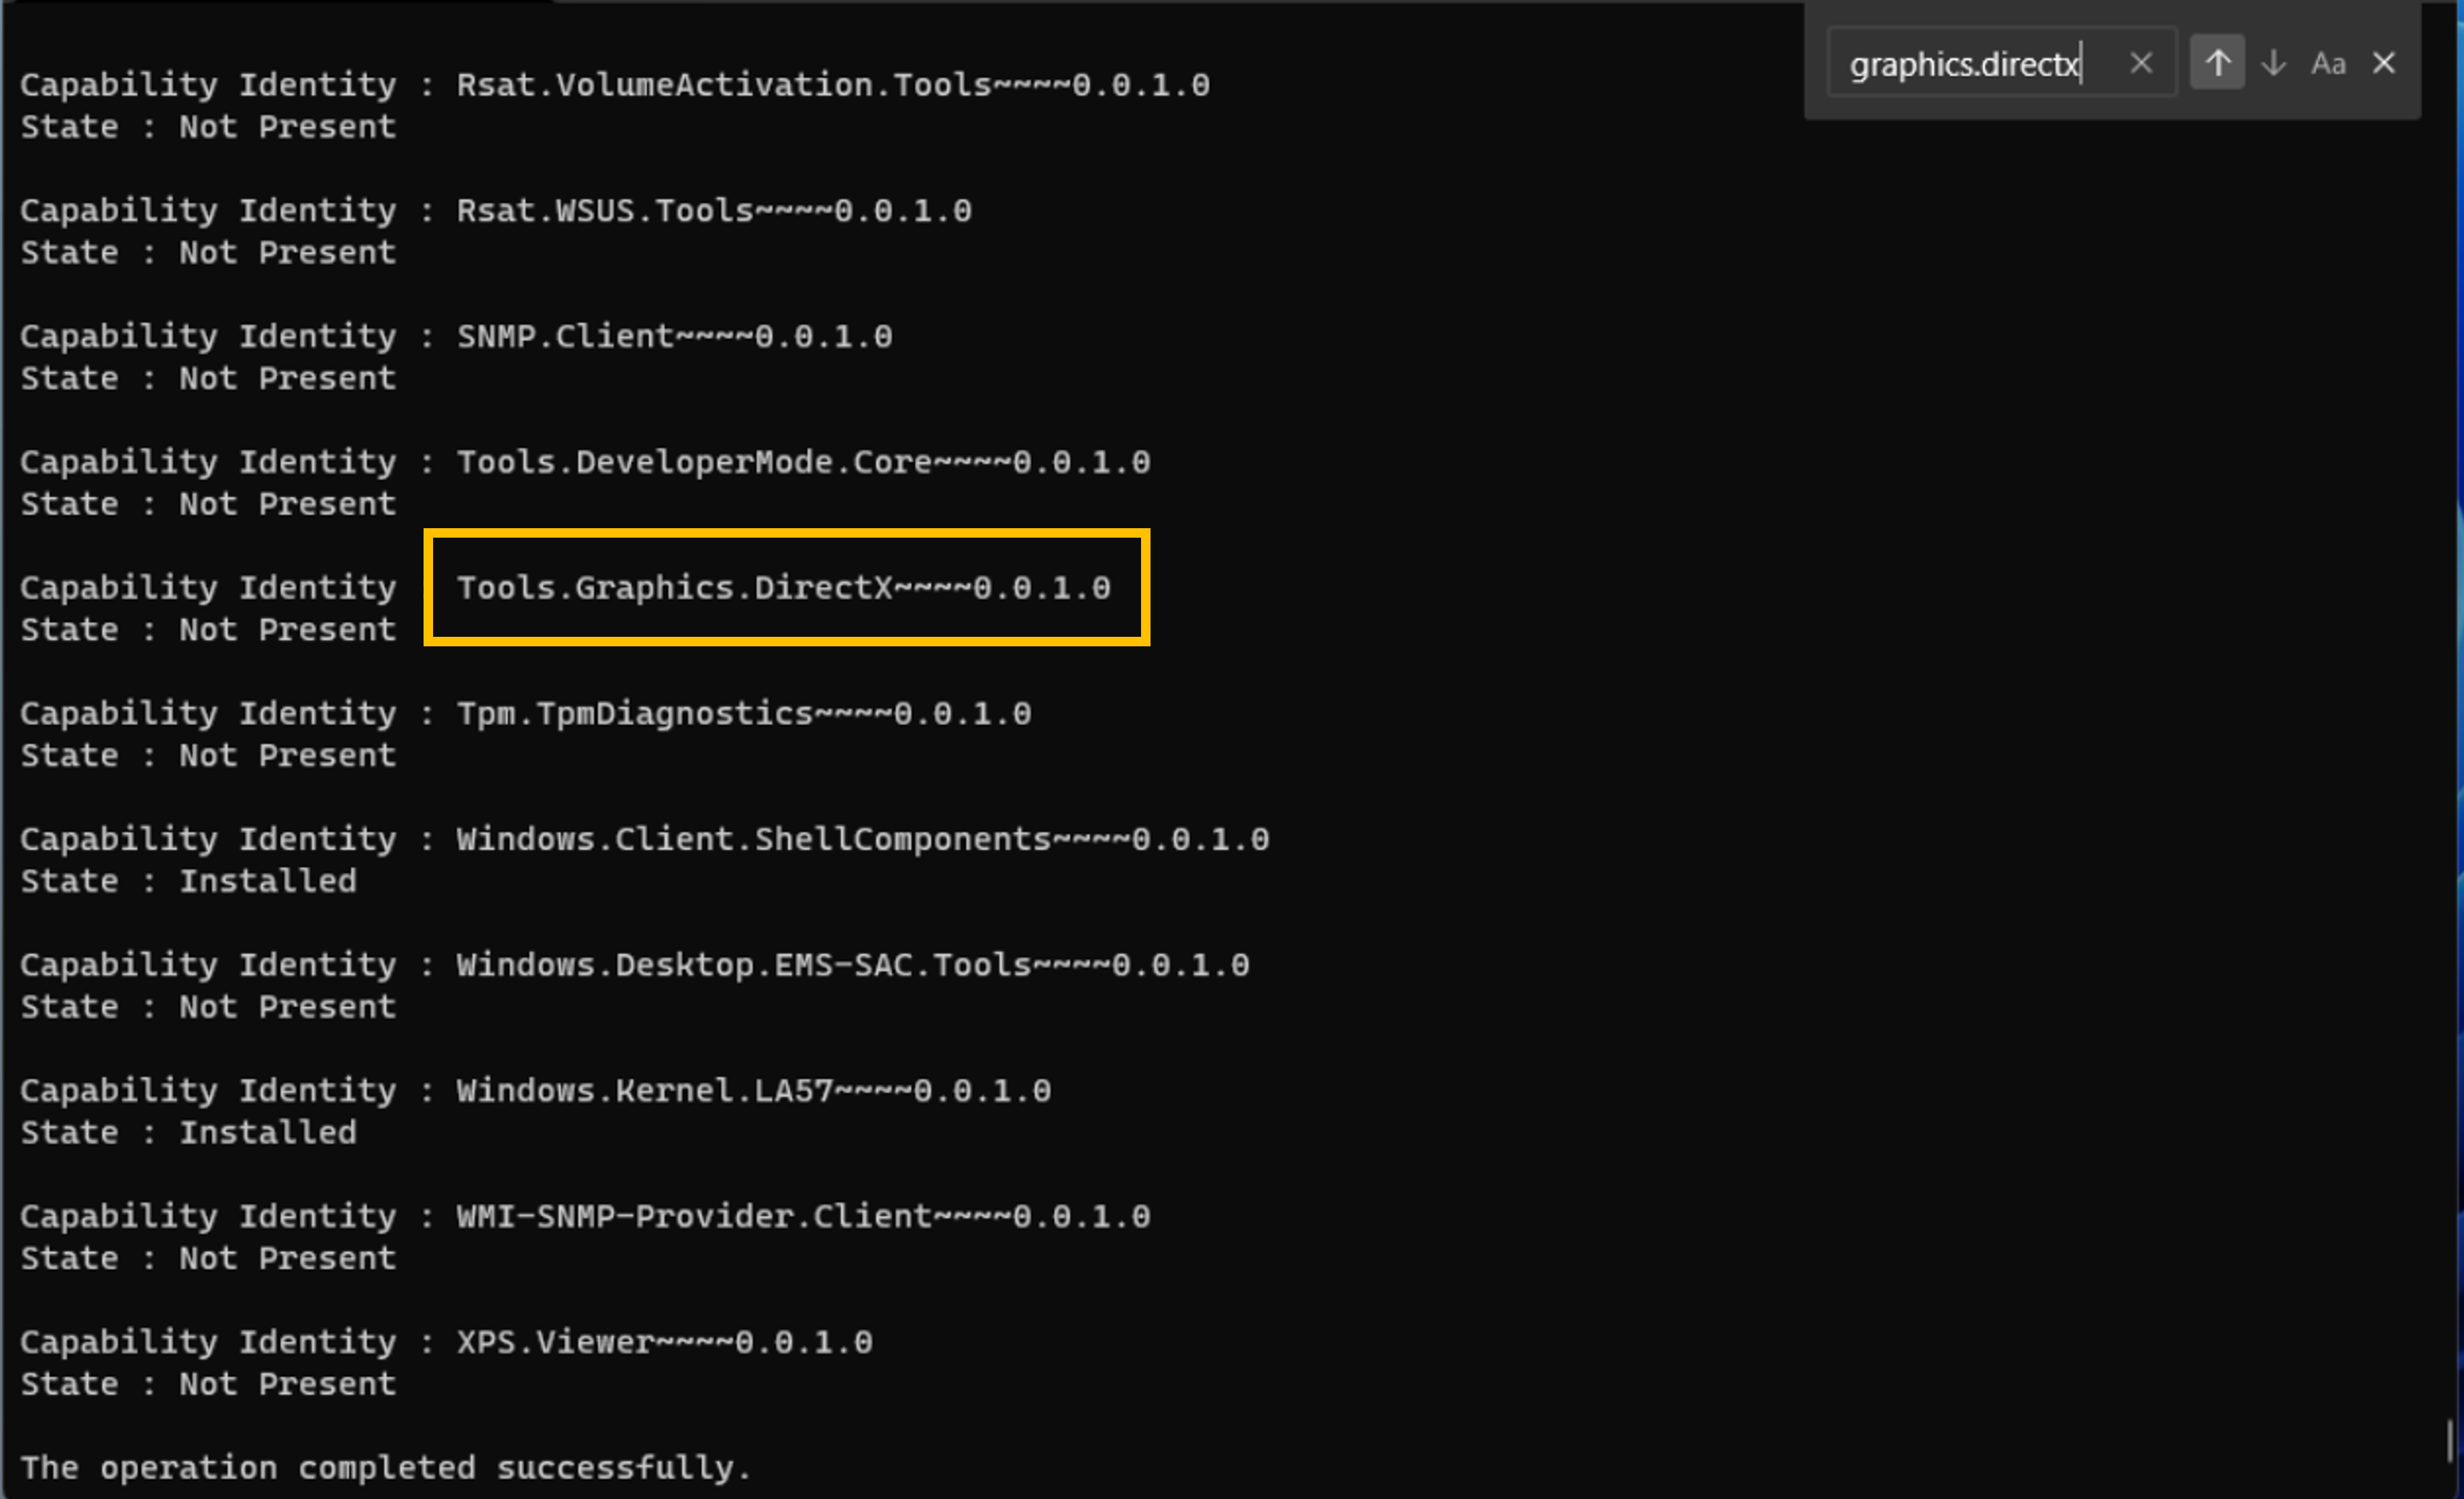
\includegraphics[width=\textwidth]{Images/1.Intro.4.3.png}
        \caption*{\lr{dism /online /Get-Capabilities}}
    \end{figure}

    از لیست نشان داده شده، موردی را که با \lr{\grayBox{Tools.Graphics.DirectX}} شروع می‌شود را پیدا کرده و کامل نام آن را کپی کنید. (ممکن است اعداد مقابل آن با عکس متفاوت باشد)

    سپس دستور زیر را وارد کنید و به جای \lr{\grayBox{<Name>}}، نامی که کپی کردید را قرار دهید.

    \begin{flushleft}
        \grayBox{Dism /Online /Add-Capability /CapabilityName:<Name>}
    \end{flushleft}

    به عنوان مثال:

    \begin{flushleft}
        \normalsize
        \grayBox{Dism /Online /Add-Capability /CapabilityName:Tools.Graphics.DirectX\textasciitilde\textasciitilde\textasciitilde\textasciitilde0.0.1.0}
    \end{flushleft}

    \begin{figure}[H]
        \centering
        \setlength{\belowcaptionskip}{-10pt}
        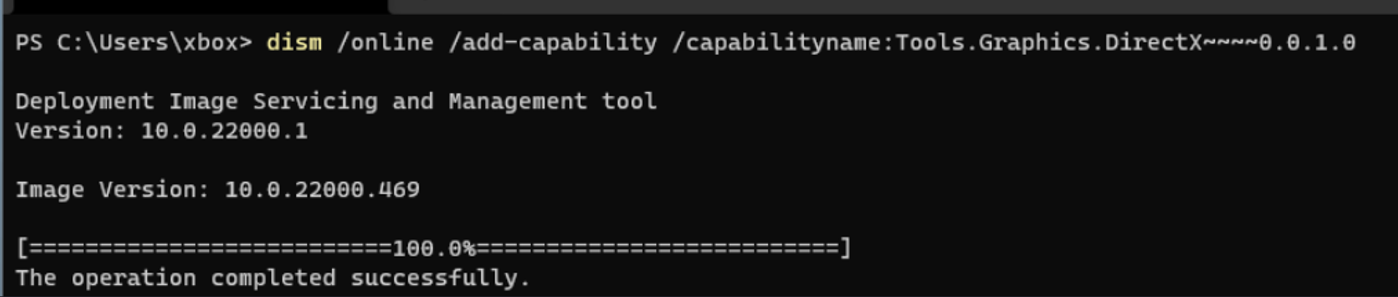
\includegraphics[width=\textwidth]{Images/1.Intro.4.4.png}
        \caption*{\lr{Dism /Online /Add-Capability /CapabilityName:Tools.Graphics.DirectX\textasciitilde\textasciitilde\textasciitilde\textasciitilde0.0.1.0}}
    \end{figure}
}
\textbf{\vspace{25pt}}

\begin{theo}{thm:pythagoras}
{
    \Large
    دقت کنید که فرآیند نصب ممکن است زمان بر باشد. همچنین دستورات \lr{Dism} به بزرگ و کوچک بودن حروف حساس نیستند.
}
\end{theo}

%--------------------------------------%
\newpage